% ARTICLE ----
% This is just here so I know exactly what I'm looking at in Rstudio when messing with stuff.
\documentclass[11pt,]{article}
\usepackage[left=1in,top=1in,right=1in,bottom=1in]{geometry}
\newcommand*{\authorfont}{\fontfamily{phv}\selectfont}
\usepackage[]{libertine}


  \usepackage[T1]{fontenc}
  \usepackage[utf8]{inputenc}




\usepackage{abstract}
\renewcommand{\abstractname}{}    % clear the title
\renewcommand{\absnamepos}{empty} % originally center

\renewenvironment{abstract}
 {{%
    \setlength{\leftmargin}{0mm}
    \setlength{\rightmargin}{\leftmargin}%
  }%
  \relax}
 {\endlist}

\makeatletter
\def\@maketitle{%
  \newpage
%  \null
%  \vskip 2em%
%  \begin{center}%
  \let \footnote \thanks
    {\fontsize{18}{20}\selectfont\raggedright  \setlength{\parindent}{0pt} \@title \par}%
}
%\fi
\makeatother




\setcounter{secnumdepth}{0}


\usepackage{graphicx,grffile}
\makeatletter
\def\maxwidth{\ifdim\Gin@nat@width>\linewidth\linewidth\else\Gin@nat@width\fi}
\def\maxheight{\ifdim\Gin@nat@height>\textheight\textheight\else\Gin@nat@height\fi}
\makeatother
% Scale images if necessary, so that they will not overflow the page
% margins by default, and it is still possible to overwrite the defaults
% using explicit options in \includegraphics[width, height, ...]{}
\setkeys{Gin}{width=\maxwidth,height=\maxheight,keepaspectratio}


\title{Estimating process-based model parameters from species
distribution data  }



\author{\Large Victor Van der Meersch
\footnote{Corresponding author - victor.vandermeersch@cefe.cnrs.fr},
Isabelle Chuine\vspace{0.05in} \newline\newline\normalsize\emph{CEFE,
Université de Montpellier, CNRS, EPHE, IRD, Montpellier, France}  }


\date{}

\usepackage{titlesec}

\titleformat*{\section}{\normalsize\bfseries}
\titleformat*{\subsection}{\normalsize\itshape}
\titleformat*{\subsubsection}{\normalsize\itshape}
\titleformat*{\paragraph}{\normalsize\itshape}
\titleformat*{\subparagraph}{\normalsize\itshape}



\usepackage{biblatex}

\addbibresource{bib/paper.bib}


\newtheorem{hypothesis}{Hypothesis}
\usepackage{setspace}


% set default figure placement to htbp
\makeatletter
\def\fps@figure{htbp}
\makeatother

\usepackage{graphicx}
\usepackage{float}
\floatplacement{figure}{H}
\usepackage[width=.9\textwidth, font=small]{caption}
\usepackage{libertine}
\usepackage[left]{lineno}
\linenumbers
\renewcommand*{\thefootnote}{\fnsymbol{footnote}}
\usepackage{booktabs}
\usepackage{longtable}
\usepackage{array}
\usepackage{multirow}
\usepackage{wrapfig}
\usepackage{float}
\usepackage{colortbl}
\usepackage{pdflscape}
\usepackage{tabu}
\usepackage{threeparttable}
\usepackage{threeparttablex}
\usepackage[normalem]{ulem}
\usepackage{makecell}
\usepackage{xcolor}

% move the hyperref stuff down here, after header-includes, to allow for - \usepackage{hyperref}

\makeatletter

\makeatother


% Add an option for endnotes. -----


% add tightlist ----------
\providecommand{\tightlist}{%
\setlength{\itemsep}{0pt}\setlength{\parskip}{0pt}}

% add some other packages ----------

% \usepackage{multicol}
% This should regulate where figures float
% See: https://tex.stackexchange.com/questions/2275/keeping-tables-figures-close-to-where-they-are-mentioned
\usepackage[section]{placeins}

% CSL environment change -----

\newlength{\cslhangindent}
\setlength{\cslhangindent}{1.5em}
\newlength{\csllabelwidth}
\setlength{\csllabelwidth}{3em}
\newenvironment{CSLReferences}[2] % #1 hanging-ident, #2 entry spacing
 {% don't indent paragraphs
  \setlength{\parindent}{0pt}
  % turn on hanging indent if param 1 is 1
  \ifodd #1 \everypar{\setlength{\hangindent}{\cslhangindent}}\ignorespaces\fi
  % set entry spacing
  \ifnum #2 > 0
  \setlength{\parskip}{#2\baselineskip}
  \fi
 }%
 {}
\usepackage{calc}
\newcommand{\CSLBlock}[1]{#1\hfill\break}
\newcommand{\CSLLeftMargin}[1]{\parbox[t]{\csllabelwidth}{#1}}
\newcommand{\CSLRightInline}[1]{\parbox[t]{\linewidth - \csllabelwidth}{#1}\break}
\newcommand{\CSLIndent}[1]{\hspace{\cslhangindent}#1}

% Last minute stuff -----
\usepackage{amssymb,amsmath} % HT @ashenkin


% Add by VV
% \usepackage[dvipsnames]{xcolor} % clash with kableExtra ?
\PassOptionsToPackage{hyphens}{url} % url is loaded by hyperref
\usepackage[unicode=true]{hyperref}
  \PassOptionsToPackage{usenames,dvipsnames}{color} % color is loaded by hyperref
\definecolor{um-red}{RGB}{233,78,82}
\definecolor{um-gray}{RGB}{114,146,162}
\definecolor{blue-sapphire}{RGB}{0, 110, 144}
\hypersetup{
    colorlinks=true,
    linkcolor=um-red,
    citecolor=um-red,
    urlcolor=um-gray,
    breaklinks=true}
\urlstyle{same} % don't use monospace font for urls
\usepackage[capitalise, nameinlink]{cleveref}




\begin{document}

% \pagenumbering{arabic}% resets `page` counter to 1
%
% \maketitle

{% \usefont{T1}{pnc}{m}{n}
\setlength{\parindent}{0pt}
\thispagestyle{plain}
{\fontsize{18}{20}\selectfont\raggedright
\maketitle  % title \par

}

{
   \vskip 13.5pt\relax \normalsize\fontsize{11}{12}
\textbf{\authorfont Victor Van der Meersch
\footnote{Corresponding author - victor.vandermeersch@cefe.cnrs.fr},
Isabelle Chuine} \hskip 15pt \emph{\small CEFE, Université de
Montpellier, CNRS, EPHE, IRD, Montpellier, France}   

}

}








\begin{abstract}

    \hbox{\vrule height .2pt width 39.14pc}

    \vskip 8.5pt % \small

\noindent \begin{enumerate}
\def\labelenumi{\arabic{enumi}.}
\item
  Two main types of species distribution models are used to project
  species range shifts in future climatic conditions: correlative and
  process-based models. Although there is some continuity between these
  two types of models, they are fundamentally different in their
  hypotheses (statistical relationships \emph{vs} cause-to-effect
  relationships) and their calibration methods (dependent \emph{vs}
  independent of the species observed distributions).
\item
  One of the main limitation to the use of process-based models is the
  difficulty to parameterize them for a very large number of species.
  Our aim was to calibrate process-based models in the same way as
  correlative models, i.e.~using the geographic distributions of
  species. We investigated the feasibility of using an evolutionary
  algorithm (called covariance matrix adaptation evolution strategy,
  CMA-ES) to calibrate these models. This method is well established in
  some fields (robotics, aerospace research, \ldots), but has never been
  used, to our knowledge, in ecology, despite its ability to deal with
  vey large space dimensions. Using tree species occurrence data across
  Europe, we adapted the CMA-ES algorithm to find appropriate values of
  model parameters. We estimated simultaneously 27 to 77 parameters of
  two process-based models simulating forest tree's ecophysiology for
  three species with varying range sizes and geographical distributions.
  We compared the performance of CMA-ES to a commonly used Approximate
  Bayesian Computation (ABC) method.
\item
  CMA-ES provided parameter estimates leading to better prediction of
  species distribution than parameter estimates based on experts
  knowledge. It was more efficient than ABC, and provided better
  parameter sets for the same amount of computation time. Predictions of
  process-based models calibrated with CMA-ES were as good as
  predictions of more simple correlative models calibrated with standard
  optimisation algorithms. Our results also revealed that some model
  parameters and processes were strongly dependent, and different
  parameter combinations could therefore lead to high model accuracy.
\item
  CMA-ES is an efficient state-of-the-art method to calibrate
  process-based models with a large number of parameters using species
  occurrence data. Inverse modelling using CMA-ES is a powerful method
  to calibrate process-based parameters which can hardly be measured.
\end{enumerate}


\vskip 8.5pt \noindent \emph{Keywords}: calibration, evolutionary
algorithm, cma-es, species distribution model, process-based model,
trees \par

    \hbox{\vrule height .2pt width 39.14pc}



\end{abstract}


\vskip -8.5pt


 % removetitleabstract

\noindent \doublespacing

\hypertarget{introduction}{%
\section{Introduction}\label{introduction}}

The speed and magnitude of projected climate changes are profoundly
affecting species distributions, ecological communities and ecosystem
processes, and numerous ecological systems are now approaching tipping
points (\protect\hyperlink{ref-Lenton2008}{Lenton \emph{et al.} 2008};
\protect\hyperlink{ref-Barnosky2012}{Barnosky \emph{et al.} 2012};
\protect\hyperlink{ref-Steffen2018}{Steffen \emph{et al.} 2018}). Large
uncertainties on the persistence and the resilience of ecosystems exist.
Ecological forecasting has now become a critical tool for managers and
decision-makers (\protect\hyperlink{ref-Urban2015}{Urban 2015}), and
robust predictive approaches are necessary to provide reliable
projections of species geographic range shifts and ecosystems
functioning (\protect\hyperlink{ref-Mouquet2015}{Mouquet \emph{et al.}
2015}). Forecasting the dynamics of ecological systems for the upcoming
decades and centuries is very difficult, because ecological systems are
extremely complex, influenced by a lot of factors and processes, and
climatic conditions with no analogous in the recent past are forecasted
to become common (\protect\hyperlink{ref-Williams2007}{Williams \emph{et
al.} 2007}; \protect\hyperlink{ref-Radeloff2015}{Radeloff \emph{et al.}
2015}; \protect\hyperlink{ref-Fitzpatrick2018}{Fitzpatrick \emph{et al.}
2018}). Ecological models have thus increased in complexity over the
last 50 years, incorporating more and more processes described with
various degrees of complexity depending on their objectives.

Nowadays, two main types of species distribution models (SDM) are used
to project species range shifts in future climatic conditions:
correlative and process-based models
(\protect\hyperlink{ref-Dormann2012}{Dormann \emph{et al.} 2012}). The
vast majority of currently used SDMs are correlative: they seek to find
statistical relationships between various environmental descriptors and
species presence and absence. They assume there is an equilibrium
between species distribution and environment (equilibrium postulate,
\protect\hyperlink{ref-Guisan2005}{Guisan \& Thuiller 2005}), and that
species niche is stable over time (niche conservatism,
\protect\hyperlink{ref-Pearman2008}{Pearman \emph{et al.} 2008}). Most
of them include a fairly large number of predictors (particularly in
machine-learning approaches), and consider flexible transformations
(linear, quadratic\ldots) and interactions between them
(\protect\hyperlink{ref-Merow2014}{Merow \emph{et al.} 2014}). Even
though some authors advocate for ``putting more biology into SDMs''
(\protect\hyperlink{ref-Higgins2012}{Higgins \emph{et al.} 2012}),
parameters have no a priori defined ecological meaning
(\protect\hyperlink{ref-Dormann2012}{Dormann \emph{et al.} 2012}) and
shape of response curves to environmental variables is generally not
constrained based on biological considerations. Although these models
are not always used correctly (\protect\hyperlink{ref-Araujo2019}{Araújo
\emph{et al.} 2019}; \protect\hyperlink{ref-Santini2021}{Santini
\emph{et al.} 2021}), their flexibility makes them an important tool in
predictive ecology (\protect\hyperlink{ref-Mouquet2015}{Mouquet \emph{et
al.} 2015}). They have been widely used especially to generate species
range projections under current and future climates (e.g.
\protect\hyperlink{ref-Guisan2005}{Guisan \& Thuiller 2005}).
Nevertheless, their ability to accurately describe the effects of
climate on species distributions has recently been questioned (e.g.
\protect\hyperlink{ref-Fourcade2018}{Fourcade \emph{et al.} 2018};
\protect\hyperlink{ref-Journe2020}{Journé \emph{et al.} 2020};
\protect\hyperlink{ref-Warren2021}{Warren \emph{et al.} 2021}). For all
these reasons, another kind of models has been developed. Process-based
models aim to translate into mathematical equations our knowledge about
the physiological and ecological processes involved in an organism's
life, such as growth, reproduction, survival, movement, and interactions
with other livebeings. Process-based models take more time to develop
and are more challenging to use, but they might provide greater
comprehension of the complexity of ecosystem dynamics and more robust
projections in novel conditions (\protect\hyperlink{ref-Evans2012}{Evans
2012}; \protect\hyperlink{ref-Zurell2016}{Zurell \emph{et al.} 2016};
\protect\hyperlink{ref-Singer2016}{Singer \emph{et al.} 2016};
\protect\hyperlink{ref-Urban2016}{Urban \emph{et al.} 2016}). A wide
variety of process-based models exists, from quite simple models (e.g.
\protect\hyperlink{ref-Kleidon2000}{Kleidon \& Mooney 2000}) to much
more complex ones (e.g. \protect\hyperlink{ref-Dufrene2005}{Dufrêne
\emph{et al.} 2005}). They all rely on an explicit representation of
causal relationships, with a direct biological interpretation
(\protect\hyperlink{ref-Connolly2017}{Connolly \emph{et al.} 2017}). The
choices about the specific processes to include into the model are made
based on theory, empirical observations and the objectives of the
research, and modeler subjectivity may play an important role. One of
the challenges is to build a model with the appropriate amount of
complexity: a too simplistic model might be unrealistic whereas a very
complex model could be far beyond our ability to understand it (because
of interconnected mechanisms) and calibrate it. Each model relies on
different hypotheses with its own balance of complexity, accuracy and
parsimony - and thus different numbers of unknown parameters to
calibrate. Generally, the parameter values are obtained both from field
or laboratory observations and experiments made by the modelers
themselves or already available in the literature, as well as from
statistical inference for each modeled process using process-specific
data.

Calibration (i.e.~parameter estimation) is a fundamental step in the
modelling process. It fixes the model in reality, and allow it to
reproduce this reality with more or less success. The result of the
calibration provides insights on the ability of the model to reproduce
and explain the reality (model predictive power). Calibration of complex
models such as process-based SDMs is time-consuming, and modelers are
often challenged by the dimension of the parameter space, the complexity
of the possible correlations among parameters, and the scarcity of
observed experimental data to calibrate them. Parameter inference can be
achieved through many methods which have been developed in the last
decades. Most of them fall into two categories: Bayesian inference or
maximum likelihood estimation. On one hand, Bayesian inference aims at
estimating parameter posterior distribution while taking into account
prior belief. On the other hand, maximum likelihood methods aim at
finding the parameters that maximize the model goodness of fit, and are
either deterministic (e.g.~Nelder-Mead method) or stochastic
(e.g.~simulated annealing, evolutionary algorithms). One of the
promising method to solve high-dimensional optimization problems is the
Approximate Bayesian Computation (ABC), which is increasingly being used
in ecological modelling (\protect\hyperlink{ref-Csillery2010}{Csilléry
\emph{et al.} 2010} ; \protect\hyperlink{ref-Beaumont2010}{Beaumont
2010}). ABC combines a computational efficient approximation of
posterior distribution with the advantages of Bayesian parameter
inference (including the quantification of parameter uncertainty), and
is thus particularly useful when numerical evaluation of the likelihood
function is computationally not possible. Recently, an other approach
belonging to the evolutionary algorithm family, called Covariance Matrix
Adaptation Evolution Strategy (CMA-ES), has been proposed
(\protect\hyperlink{ref-Hansen2001}{Hansen \& Ostermeier 2001}). One of
the advantage of CMA-ES is its ability to cumulate information over
iterations in order to adapt its own parameters (in particular the
covariance matrix), which makes it more robust to noise. CMA-ES is
especially performant for non-separable problems (i.e.~when the model
parameters are dependent) and large search space. This method has been
successfully applied in various fields such as aerospace (e.g.
\protect\hyperlink{ref-Collange2010}{Collange \emph{et al.} 2010}),
optics (e.g. \protect\hyperlink{ref-Gagne2008}{Gagné \emph{et al.}
2008}), and robotics (e.g. \protect\hyperlink{ref-Hill2020}{Hill
\emph{et al.} 2020}). CMA-ES is acknowledged to be one of the most
efficient approaches in continuous black-box optimization
(\protect\hyperlink{ref-Hansen2010}{Hansen \emph{et al.} 2010}) but to
our knowledge has never been used in ecology.

Here we explored the feasibility and interests of calibrating
process-based SDMs with CMA-ES using species occurrence data as
correlative SDMs do. We focused on two forest process-based models of
varying levels of complexity to evaluate the ability of CMA-ES to
calibrate such models and compare its performance relatively to the more
widely used ABC method. The two models are PHENOFIT (27 to 36
parameters, \protect\hyperlink{ref-Chuine2001}{Chuine \& Beaubien 2001})
and CASTANEA (77 parameters, \protect\hyperlink{ref-Dufrene2005}{Dufrêne
\emph{et al.} 2005}). Each model also emphasizes different ecological
processes: while PHENOFIT focuses on phenology and how it relates to
survival and reproduction, CASTANEA focuses on carbon and water cycles.
We aimed to assess the ability of CMA-ES to calibrate these
process-based models, to identify the limits of this method, and to
compare its efficiency with an ABC algorithm commonly used among
ecologists. To this end, we calibrated the models in the same way as
correlative models do (fitted process-based models \emph{sensu}
\protect\hyperlink{ref-Dormann2012}{Dormann \emph{et al.}}
(\protect\hyperlink{ref-Dormann2012}{2012})), that is to say, using the
geographic distributions of species, and compare their efficiency to
that obtained with classical calibration, i.e.~direct measurement of the
parameters or statistical inference of the different submodels using
data for each modelled process. We focused on three European common tree
species, with different range extent and ecological preferences in order
to evaluate the algorithms performance in various geographical and
climatic conditions. European beech (\emph{Fagus sylvatica L.}) is one
of the most widely distributed broadleaved tree in Europe (from southern
Sweden to Sicily and from Spain to northwest Turkey), holm oak
(\emph{Quercus ilex L.}) is an evergreen broadleaved tree native of the
Mediterranean region, and silver fir (\emph{Abies alba Mill.}) is a
coniferous tree which mainly occurs in mountain forests of Central
Europe and some parts of Southern and Eastern Europe.

\hypertarget{methods}{%
\section{1. Material and methods}\label{methods}}

\hypertarget{pbmodels}{%
\subsection{1.1. Process-based models}\label{pbmodels}}

All versions of the models used for this study are coded in Java and
distributed by the \href{https://capsis.cirad.fr/capsis/home}{CAPSIS}
platform.

PHENOFIT is a process-based species distribution model for forest tree
species which focuses on phenology. It relies on the principle that the
distribution of a tree species depends mainly on the synchronization of
its timing of development to the local climatic conditions
(\protect\hyperlink{ref-Chuine2001}{Chuine \& Beaubien 2001}). It is
composed of several submodels, including phenology models for leaves,
flowers and fruits, and stress resistance models. It simulates the
fitness (survival and reproductive success) of an average individual
using daily meteorological data, soil water holding capacity and species
specific parameters (see \protect\hyperlink{appendixA}{Appendix A} for
details). PHENOFIT has been validated for several North American and
European species by comparing their known distribution to the modelled
fitness (e.g. \protect\hyperlink{ref-Morin2007}{Morin \emph{et al.}
2007}; \protect\hyperlink{ref-Saltre2013}{Saltré \emph{et al.} 2013};
\protect\hyperlink{ref-Duputie2015}{Duputié \emph{et al.} 2015};
\protect\hyperlink{ref-Gauzere2020}{Gauzere \emph{et al.} 2020}).

CASTANEA is an ecophysiological process-based model which simulates
carbon and water fluxes in forests
(\protect\hyperlink{ref-Dufrene2005}{Dufrêne \emph{et al.} 2005}). The
model simulates the ecosystem as an average tree with six compartments
(leaves, branches, stem, coarse roots, fine roots and reserves). It is
much more complex than PHENOFIT, with several processes described and
computed, such as photosynthesis, stomatal opening, maintenance and
growth respiration, transpiration, and carbon allocation (see
\protect\hyperlink{appendixA}{Appendix A} for details). CASTANEA
requires daily meteorological variables and soil characteristics. The
model has been initially validated at stand scale for beech
(\protect\hyperlink{ref-Davi2005}{Davi \emph{et al.} 2005}), and was
then successfully applied to other European species (e.g.
\protect\hyperlink{ref-Davi2006}{Davi \emph{et al.} 2006};
\protect\hyperlink{ref-Delpierre2012}{Delpierre \emph{et al.} 2012};
\protect\hyperlink{ref-Davi2017}{Davi \& Cailleret 2017}).

\hypertarget{data}{%
\subsection{1.2. Data for the calibration}\label{data}}

\hypertarget{climatedata}{%
\subsubsection{1.2.1. Climate and soil data}\label{climatedata}}

Raw climatic variables were extracted from ERA5-Land hourly dataset
(\protect\hyperlink{ref-Sabater2019}{Muñoz Sabater 2019},
\protect\hyperlink{ref-Sabater2021}{2021}) from 1970 to 2000, at a
spatial resolution of 0.1 degree in latitude and longitude. We
calculated the daily mean values of the following variables used by
PHENOFIT and CASTANEA: minimum, mean and maximum daily temperatures,
mean dewpoint temperature, daily precipitation, daily global radiation
and daily mean wind speed. We computed the daily relative humidity with
the ratio of vapor pressure and saturation vapor pressure (both
calculated with Clausius-Clapeyron equation) using \emph{humidity} R
package (\protect\hyperlink{ref-Cai2019}{Cai 2019}). Daily potential
evapotranspiration was calculated with Penman--Monteith equation (FAO
standard of hypothetical grass reference surface) using a slightly
modified version of the \emph{ET()} function in
\emph{Evapotranspiration} R package (\protect\hyperlink{ref-Guo2016}{Guo
\emph{et al.} 2016}).

Water content at field capacity and wilting point data were extracted
from EU-SoilHydroGrids (\protect\hyperlink{ref-Toth2017}{Tóth \emph{et
al.} 2017}) which is at 1km resolution. Percentage of sand, silt and
clay particles, percentage of coarse fragments, bulk density and soil
depth were extracted from SoilGrids250m
(\protect\hyperlink{ref-Hengl2017}{Hengl \emph{et al.} 2017}) at a 250m
resolution. These data (except for soil depth) are provided at seven
soil depths, so we summarized them (weighted sum or weighted mean)
taking into account each layer width and total soil depth. Finally, all
variables were upscaled at the ERA5-Land spatial resolution 0.1°.

\hypertarget{occurrencedata}{%
\subsubsection{1.2.2. Tree occurrences in Europe}\label{occurrencedata}}

Sources of occurrence data are known to differ even for common European
trees (\protect\hyperlink{ref-Duputie2014}{Duputié \emph{et al.} 2014})
and this makes it quite challenging to gather comprehensive data at a
sufficient spatial resolution all over Europe. The occurrence data we
used essentially rely on the EU-Forest dataset
(\protect\hyperlink{ref-Mauri2017}{Mauri \emph{et al.} 2017}) which
benefits from inventory and monitoring programmes implemented in most
European countries. As EU-Forest is limited to forest ecosystems, we
completed it with presence records extracted from the Global
Biodiversity Information Facility (\protect\hyperlink{ref-GBIF2022}{GBIF
2022}, see \protect\hyperlink{appendixB}{Appendix B} for all download
links) but removing observations outside natural species ranges as
defined by Atlas Flora Europeae (AFE,
\protect\hyperlink{ref-AFE2005}{Jalas \& Suominen 1972--2005}) and
EuroVegMap (\protect\hyperlink{ref-EVM2003}{Bohn \emph{et al.} 2003}).
By doing so, we also included occurrences of isolated native trees
living outside forests, excluding records from arboreta or gardens where
the species would have been planted as an exotic. For holm oak, we also
added occurrence records in the Mediterranean Basin from the WOODIV
database (\protect\hyperlink{ref-Monnet2021}{Monnet \emph{et al.}
2021}), leaving out EU-Forest and GBIF records we had already gathered.
We upscaled all species records at the ERA5-Land resolution (i.e.~0.1°
cell, see \protect\hyperlink{climatedata}{1.2.1. Climate data}). We
finally obtained 21458 occurrence cells for beech, 6653 for holm oak and
5385 for silver fir (see \protect\hyperlink{appendixB}{Appendix B} for
details).

All the datasets described above are presence-only data. Therefore, we
generated cells where species are supposed to be absent,
i.e.~pseudo-absence cells. In order to avoid as far as possible creating
false absence data, we used EU-Forest cells where the species is not
reported present as pseudo-absence cells. We assumed that national
forest inventories were exhaustive (which is not true since only
specific forest plots in a 0.1° cell are monitored). We obtained 25423
absence cells for beech, 37931 for holm oak and 38365 for silver fir
(see \protect\hyperlink{appendixC}{Appendix C}).

We selected subsets of 2000 points (1000 presences and 1000
pseudo-absences) in order to reduce computational costs. For each
species, we generated ten presence clusters of similar bioclimatic
conditions based on annual climate normals computed with R package
\emph{dismo} (\protect\hyperlink{ref-Hijmans2021}{Hijmans \emph{et al.}
2021}) and ERA5-Land variables. In each cluster, we randomly sampled a
number of cells where the species is present proportional to the total
number of a number of cells where the species is present in the cluster.
The aim of this stratified random sampling was to make sure that all
species environmental preferences were proportionally represented. We
then randomly sampled the same number of pseudo-absence cells (see
\protect\hyperlink{appendixB}{Appendix B} for details).

\hypertarget{model-calibration}{%
\subsection{1.3. Model calibration}\label{model-calibration}}

\hypertarget{covariance-matrix-adaptation-evolution-strategy-principles}{%
\subsubsection{1.3.1. Covariance Matrix Adaptation Evolution Strategy
principles}\label{covariance-matrix-adaptation-evolution-strategy-principles}}

Covariance Matrix Adaptation Evolution Strategy (CMA-ES) is widely
accepted as a robust optimization algorithm for non-linear, non-convex,
as well as non-separated optimization problems in continuous domain
(\protect\hyperlink{ref-Hansen1996}{Hansen \& Ostermeier 1996};
\protect\hyperlink{ref-Hansen2001}{Hansen \& Ostermeier 2001};
\protect\hyperlink{ref-Hansen2006}{Hansen 2006}). It is based on the
principle of evolutionary biology, via recombination, mutation and
selection of the most fit individuals (i.e.~parameter sets providing the
best predictions). At each iteration:\\
- \(\lambda\) individuals are evaluated, i.e.~model runs \(\lambda\)
times with \(\lambda\) different parameter sets and the objective
function is evaluated\\
- the best \(\mu\) indivuals are selected\\
- the weighted mean individual \(m\) is computed (mean of the best
\(\mu\) parameter sets weighted by their objective function value) -
covariance matrix \(C\) and step size \(\sigma\) are updated (with
information accumulated over several consecutive iterations)\\
- new \(\lambda\) individuals are sampled in a normal distribution
\(\mathcal{N}(m, \sigma C)\), with both recombination (via the favorite
solution \(m\)) and mutations (via the perturbations \(\sigma C\))\\
One of the strength of this approach lies in the combination of
rank-\(\mu\)-update, where prior information from previous generations
is exploited (mean of the previous covariance matrices, with a higher
weight for recent generations), and cumulation, where correlations
between generations are retained in an evolution path (sum of
consecutive steps), to update the covariance matrix at each step (see
\protect\hyperlink{ref-Hansen2016}{Hansen 2016} for a detailed
description of the algorithm).

\hypertarget{cma-es-in-practice}{%
\subsubsection{1.3.2. CMA-ES in practice}\label{cma-es-in-practice}}

One of the advantages of CMA-ES is that it does not require a complex
parameter tuning: as best parameter values at a given time of the
optimization process might no longer be efficient later, CMA-ES
implements an internal adaptation of its parameters. We only chose the
population size \(\lambda\), depending on the optimization problem
complexity (\(\mu\) was set to \(\lambda/2\)). The default recommended
value for \(\lambda\) is \(4 + 3 ln(N)\), where \(N\) is the number of
parameters to calibrate (i.e.~\(\lambda \in [14,17]\) in our case). We
set \(\lambda = 20\), in order to improve the global search capability
(\protect\hyperlink{ref-Hansen2004}{Hansen \& Kern 2004}) and take
advantage of the computation power at our disposal. All model parameters
were linear scaled into \([0;10]\) so that the same standard deviation
can be applied to all parameters: here we chose \(\sigma = 2\) (see
\href{https://cma-es.github.io/cmaes_sourcecode_page.html\#practical}{Nikolaus
Hansen personal website} for practical hints on variable encoding). Our
stopping criterion for the optimization procedure was the budget,
i.e.~the number of model runs.

For an easier use and the sake of reproducibility, we chose to use a
pure R implementation of CMA-ES available in the R package \emph{cmaes}
(\protect\hyperlink{ref-Trautmann2011}{Trautmann \emph{et al.} 2011}).
The function \emph{cma\_es()} enables us to do \(\lambda\) function
evaluations in parallel so as to substantially reduce computation time.
It also allows us to define lower and upper bound constraints, by
penalising individual fitness (i.e.~objective function value) if it
violates the boundaries. We customized the \emph{cma\_es()} function to
add an option to define death penalty constraints (rejection of the
infeasible individual who is sampled again), in order to define a range
of ecologically possible solutions in terms of inequality constraints
between parameters (see \protect\hyperlink{appendixD}{Appendix D} for
details about boundaries and constraints handling). Death penalty is the
easiest way to handle constraints when the feasible region is fairly
large, but it is not perfect as there is no use of information from
infeasible points.

In the spirit of species distribution modelling, the objective function
for the calibration was the area under the receiver operating
characteristic curve (AUC), evaluated against a subsets of 2000 points
(see \protect\hyperlink{occurrencedata}{1.2.2. Tree occurrences}).
Although AUC has been criticized as an imperfect measure of model
performance (\protect\hyperlink{ref-Lobo2008}{Lobo \emph{et al.} 2008};
\protect\hyperlink{ref-Leroy2018}{Leroy \emph{et al.} 2018}), we used it
as objective function because our goal here was only to calibrate models
by maximizing discriminating capacity (i.e.~potential to correctly
classify presences and absences) with a threshold-independent measure.
We used the \emph{AUC} R package
(\protect\hyperlink{ref-Ballings2013}{Ballings \& Van den Poel 2013}),
and chose the two following model output variables as proxies of
classification probabilities (i.e.~used to determine if the species can
be present or not): fitness index for PHENOFIT and carbon reserves for
CASTANEA (see \protect\hyperlink{appendixA}{Appendix A}).

We implemented the CMA-ES calibration on two computing clusters:
GenOuest from IRISA-INRIA
(\href{https://www.genouest.org}{genouest.org}) and TGCC (\emph{Très
Grand Centre de Calcul}) from CEA
(\href{http://www-hpc.cea.fr/fr/complexe/tgcc.htm}{hpc.cea.fr}). As the
models are coded in Java (see \protect\hyperlink{pbmodels}{1.1
Process-based models}), they need a process of deallocating memory
handled by a \emph{garbage collector}. For PHENOFIT, each function
evaluation (i.e.~each model simulation) was run on a 2-core computing
unit in order to have enough computing resources for both simulation and
garbage collection. We thus needed twice as many cores as functions
evaluated in parallel. CASTANEA model requires a fairly high computation
time, so we used a nested parallelism distribution, where each parallel
simulation was distributed on 4 computing units. We thus used 4 times as
many cores as functions evaluated in parallel, plus some extra cores for
garbage collection. We used R package \emph{future}
(\protect\hyperlink{ref-Bengtsson2021}{Bengtsson 2021}) for parallel
processing.

\begin{table}

\caption{\label{tab:modelstable}Summary of model calibration settings. Average runtime was assessed on the GenOuest cluster.}
\centering
\begin{tabu} to \linewidth {>{\raggedright}X>{\raggedright}X>{\raggedright}X>{\raggedright}X>{\raggedright}X>{\raggedright}X>{\raggedright}X}
\toprule
Model & Output variable of interest & Number of parameters calibrated & Population size $\lambda$ & Number of cores & Memory & Average runtime\\
\midrule
PHENOFIT & Fitness index & $[27;36]$ & $20$ & $40$ & $80$ Go & $\sim 24$ hours\\
\addlinespace
CASTANEA & Carbon reserves & $77$ & $20$ & $100$ & $120$ Go & $\sim 20$ days\\
\bottomrule
\end{tabu}
\end{table}

Regarding PHENOFIT model, we calibrated ten times each species parameter
set using CMA-ES algorithm, with 5 repetitions on 2 random subsets of
presences/pseudo-absences (see \protect\hyperlink{occurrencedata}{1.2.2.
Tree occurrences}), except for beech. In the latter case, we ran 10
repetitions on 10 subsets (i.e.~100 calibrations) to investigate both
the effect of subsampling and the effect of stochasticity on the
calibration performance of CMA-ES. Since CASTANEA computing time was
much higher (see \autoref{tab:modelstable}), we ran only two calibration
for each species (on 2 different random subsets).

\hypertarget{approximate-bayesian-computation}{%
\subsubsection{1.3.3. Approximate Bayesian
Computation}\label{approximate-bayesian-computation}}

In order to provide elements of comparison between CMA-ES and an other
widely used and effective optimization algorithm, we also implemented an
Approximate Bayesian Computation (ABC) method. We chose ABC because it
is well established in ecology (e.g.
\protect\hyperlink{ref-Hartig2014}{Hartig \emph{et al.} 2014};
\protect\hyperlink{ref-Lagarrigues2015}{Lagarrigues \emph{et al.} 2015};
\protect\hyperlink{ref-Vaart2015}{Vaart \emph{et al.} 2015};
\protect\hyperlink{ref-Gardner2020}{Gardner \emph{et al.} 2020}).
Several versions of ABC exist, but here we only explore the most
accessible version, simple rejection. We chose this version because it
does not require a tedious parameter tuning, and it is therefore as easy
as CMA-ES to apply to various calibration problems.\\
ABC rejection involves running the model a large number of times, with
parameters randomly sampled from their prior distributions, and then
accepting the simulations closest to the observed data. These retained
simulations are then used to draw the posterior distributions of the
model's parameters given the data. We used uniform priors with the same
lower and upper bounds than CMA-ES. We ran the model the same number of
times as CMA-ES (i.e.~same number of objective function evaluations) and
we obtain the same computation time. Therefore, we had a fair comparison
of the performance of the two algorithms.\\
We ran 30 ABC calibrations (10 repetitions on 3 subsets) of PHENOFIT for
beech in order to be able to make a robust comparison with CMA-ES. To
avoid getting a beech specific comparison, we also ran 10 ABC
calibrations (5 repetitions on 2 subsets) of PHENOFIT for holm oak (see
\protect\hyperlink{appendixE}{Appendix E}).

\hypertarget{results}{%
\section{2. Results}\label{results}}

\hypertarget{calibration-results}{%
\subsection{2.1. Calibration results}\label{calibration-results}}

Calibrations using species distribution data, either CMA-ES or ABC, are
thereafter called backward calibrations, and calibrations based on
expert knowledge, observations and measurements of the processes
modelleds are called forward calibrations.

CMA-ES calibration of PHENOFIT model allows an average 17.2\% increase
of AUC across the three species compared to forward calibration
(\hyperref[fig:phenofitmaps]{Figure 1}). The maximum increase is
obtained for silver fir, from 0.72 to 0.9 (25\%).\\
CMA-ES calibration of CASTANEA allows an average 23.7 \% increase of AUC
compared to forward calibration (\hyperref[fig:castaneamaps]{Figure 2}),
and a maximum increase obtained for holm oak (34.7\%).

\begin{figure}[H]

{\centering 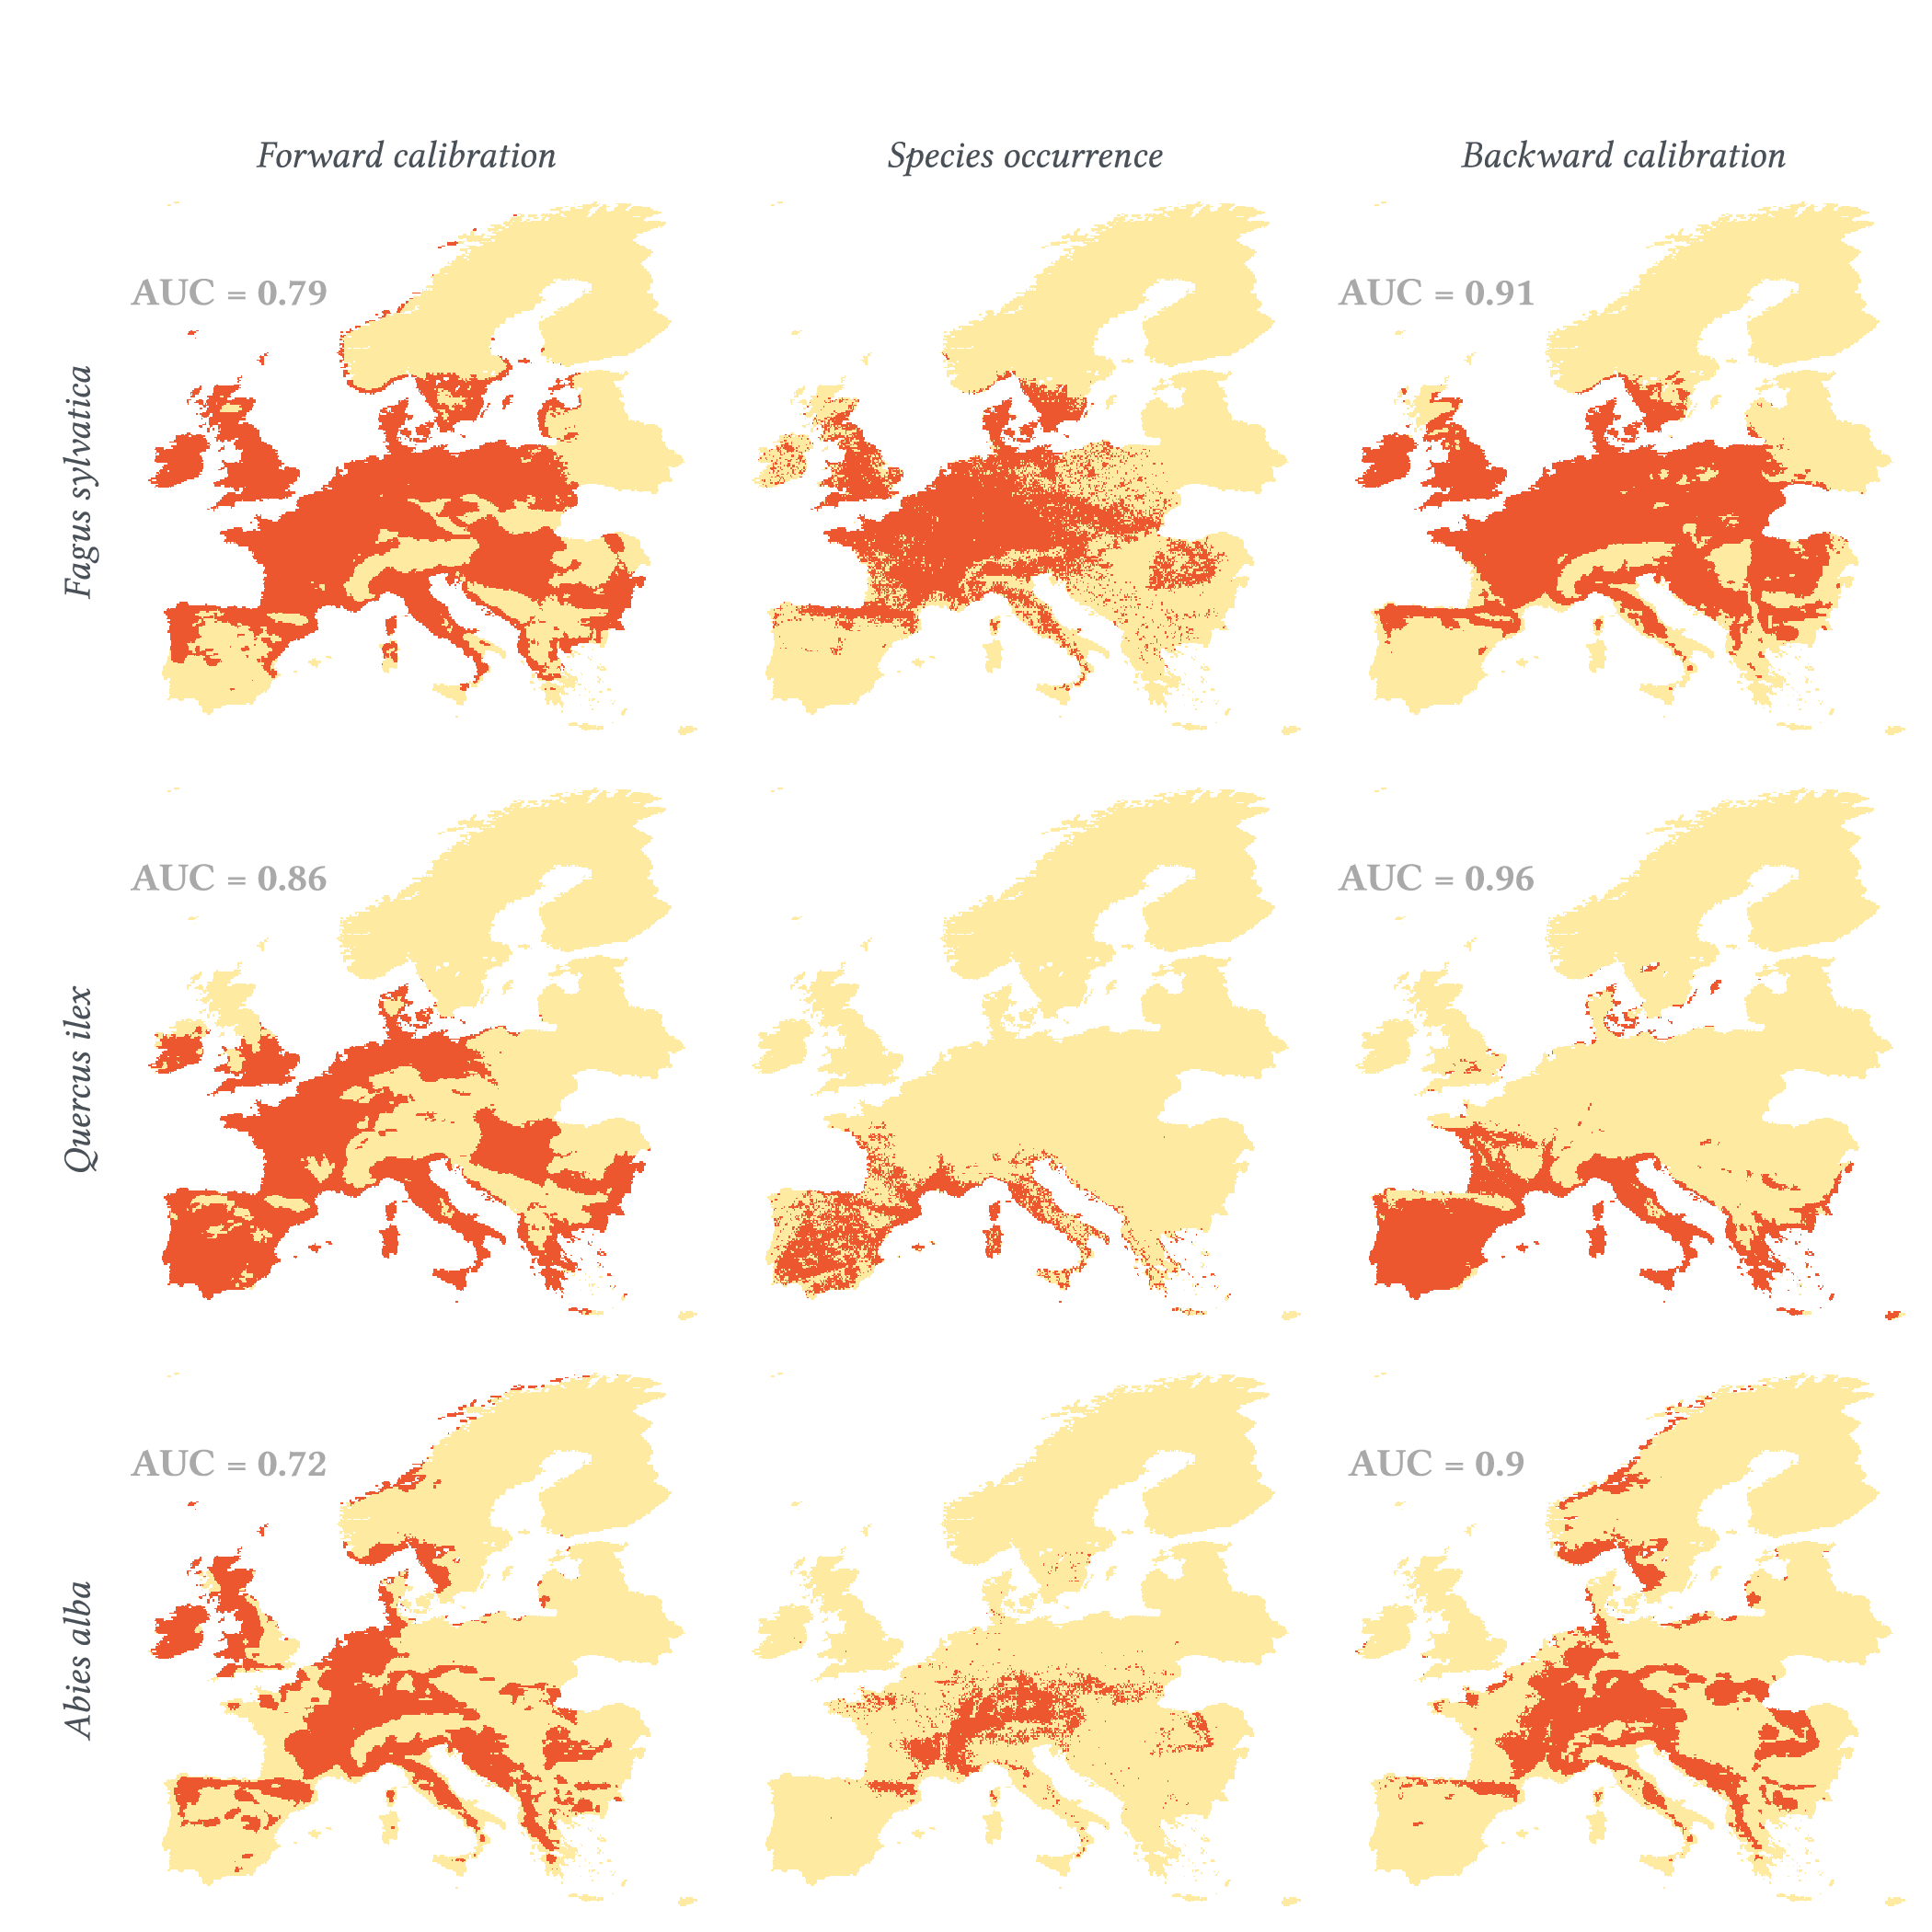
\includegraphics{figs/phenofitmaps} 

}

\caption{Species distribution maps obtained with PHENOFIT forward and backward calibrations, compared with observed species occurrences. Optimal threshold to dichotomize model predicted fitness index in presence/absence is the Youden index-based cut-off point. Note that models predict species climatic niche which is larger than the realized niche that corresponds to species presence map.}\label{fig:phenofitmaps}
\end{figure}

\begin{figure}[H]

{\centering 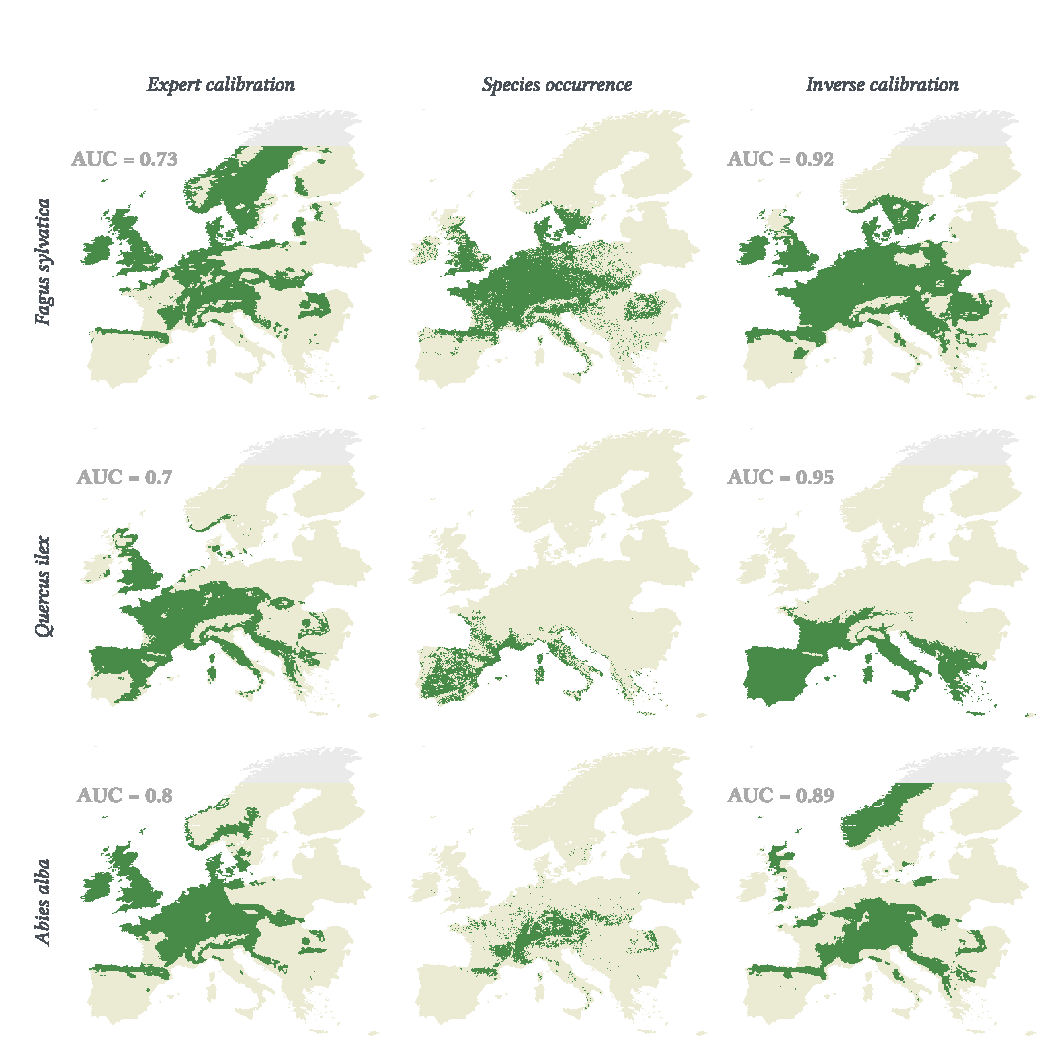
\includegraphics{figs/castaneamaps} 

}

\caption{Species distribution maps obtained with CASTANEA forward and backward calibrations, compared with observed species occurrences. Optimal threshold to dichotomize model predicted carbon reserves in presence/absence is the Youden index-based cut-off point. Note that models predict species climatic niche which is larger than the realized niche that corresponds to species presence map.}\label{fig:castaneamaps}
\end{figure}

\hypertarget{impacts-of-subsampling-and-calibration-stochasticity}{%
\subsection{2.2. Impacts of subsampling and calibration
stochasticity}\label{impacts-of-subsampling-and-calibration-stochasticity}}

\hypertarget{variability-of-calibration-performance}{%
\subsubsection{2.2.1. Variability of calibration
performance}\label{variability-of-calibration-performance}}

\begin{figure}[H]

{\centering 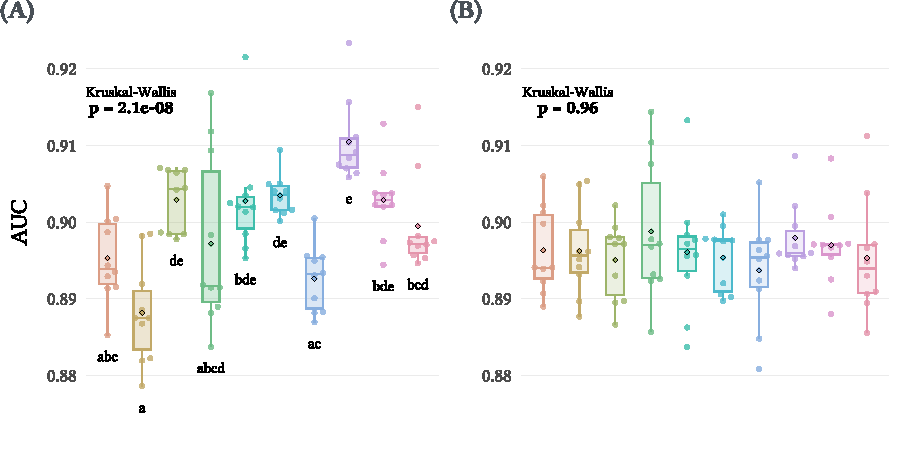
\includegraphics{figs/cmaesrepAUCcal} 

}

\caption{\label{fig:cmaesrepAUCcal} Effects of data sub-sampling and stochasticity on CMA-ES calibration using the PHENOFIT model for beech: \textbf{(A)} calibration AUC (calculated only with calibration cells) and \textbf{(B)} total AUC (calculated with all presence/absence cells). Each color is a different sub-sampling of occurrence data, each point is a calibration run. Diamonds (with black border) are mean AUC values. On \textbf{(A)}, the grouping letters represent the multiple comparisons with pairwise Dunn’s tests.}\label{fig:cmaesrepAUCcal}
\end{figure}

The 100 calibrations of the PHENOFIT model realized for beech showed
that random data subsampling had an effect on the final objective
function value (i.e.~the AUC computed on the 2000 calibration points).
Kruskal-Wallis test was significant (p = 2.1e-08), meaning that at least
one subset provided better AUC during calibration. According to Dunn's
tests, 11 pairwise comparisons out of 45 were significant
(\hyperref[fig:cmaesrepAUCcal]{Figure 3.A.}). The calibration AUC ranged
from 0.879 to 0.923 over all subsets, with a mean value of 0.9.

However, more importantly, the repetition of calibrations on different
subsets had no significant impact on the total AUC computed on all
presence/absence points (Kruskal-Wallis test, p = 0.96). Thus, no subset
led to an overall better prediction of the species distribution (see
\hyperref[fig:cmaesrepAUCcal]{Figure 3.B.}). The total AUC ranged from
0.881 to 0.914, with a mean value of 0.896. \newline

\hypertarget{non-identifiability-of-parameters}{%
\subsubsection{2.2.2. Non-identifiability of
parameters}\label{non-identifiability-of-parameters}}

We found a high variability in the parameter estimates of the leaf
unfolding date submodel of PHENOFIT after 100 calibrations
(\hyperref[fig:unfoldingplots]{Figure 4.A.}). For example, the critical
amount of chilling \(C_{crit}\) required to break bud dormancy and the
critical amount of forcing \(F_{crit}\) required to break bud ranged
from 1.02 to 149.96 and from 1.5 to 79.26 respectively, with a mean
value of 51.52 and 38.78. Their coefficient of variations were 126.7\%
and 51.9\% respectively. Kendall correlation coefficient between
\(C_{crit}\) and the threshold temperature of the response function to
temperature during dormancy \(T_b\) is 0.64 (\(p <\) 0.001). Kendall
correlation coefficient between \(F_{crit}\) and the mid-response
temperature \(T_{50}\) is -0.55 (\(p <\) 0.001).

\begin{figure}[H]

{\centering 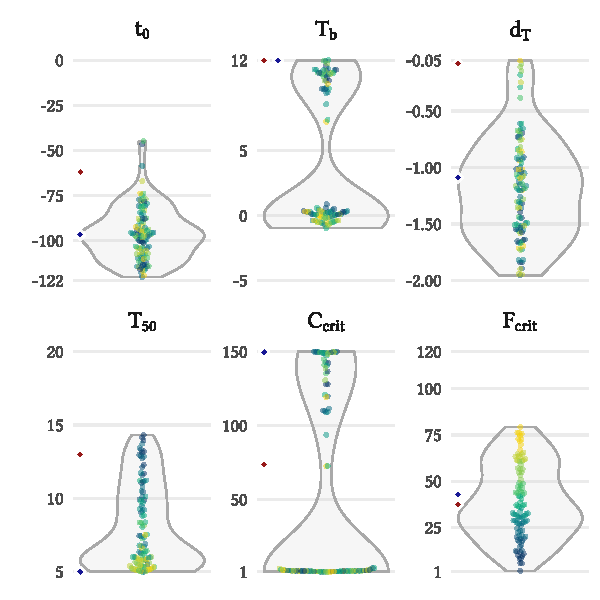
\includegraphics{figs/unfoldingplots} 

}

\caption{Effects of stochasticity of \textbf{(A)} CMA-ES and \textbf{(B)} ABC calibrations on PHENOFIT leaf unfolding model parameter values for beech. Y-axis limits are lower and upper bounds used during calibration. Each point is a calibrated parameter value, color gradient is based on $F_{crit}$ values. Red diamonds are parameter values obtained with classical (forward) calibration, blue ones are parameter values obtained with the best backward calibration.}\label{fig:unfoldingplots}
\end{figure}

\hypertarget{comparing-cma-es-and-abc-efficiency}{%
\subsection{2.3. Comparing CMA-ES and ABC
efficiency}\label{comparing-cma-es-and-abc-efficiency}}

The mean calibration AUC and total AUC obtained for beech with CMA-ES
(0.899 and 0.896 respectively) were only slightly higher than those
obtained with ABC (0.872 and 0.869). The best total AUC obtained with
CMA-ES was 0.913, a higher value than the best solution obtained with
ABC, 0.876. According to Mann--Whitney tests, the distributions of AUC
measures between the two methods with the three different occurrence
subsets differed significantly
(\hyperref[fig:comparisonABCCMAES]{Figure 5}). The outperformance of
CMA-ES compared with ABC was the same for holm oak (see Figure E.1. in
\protect\hyperlink{appendixE}{Appendix E}). Both methods result in a
high variability in the parameter estimates
(\hyperref[fig:unfoldingplots]{Figure 4}) .

\begin{figure}[H]

{\centering 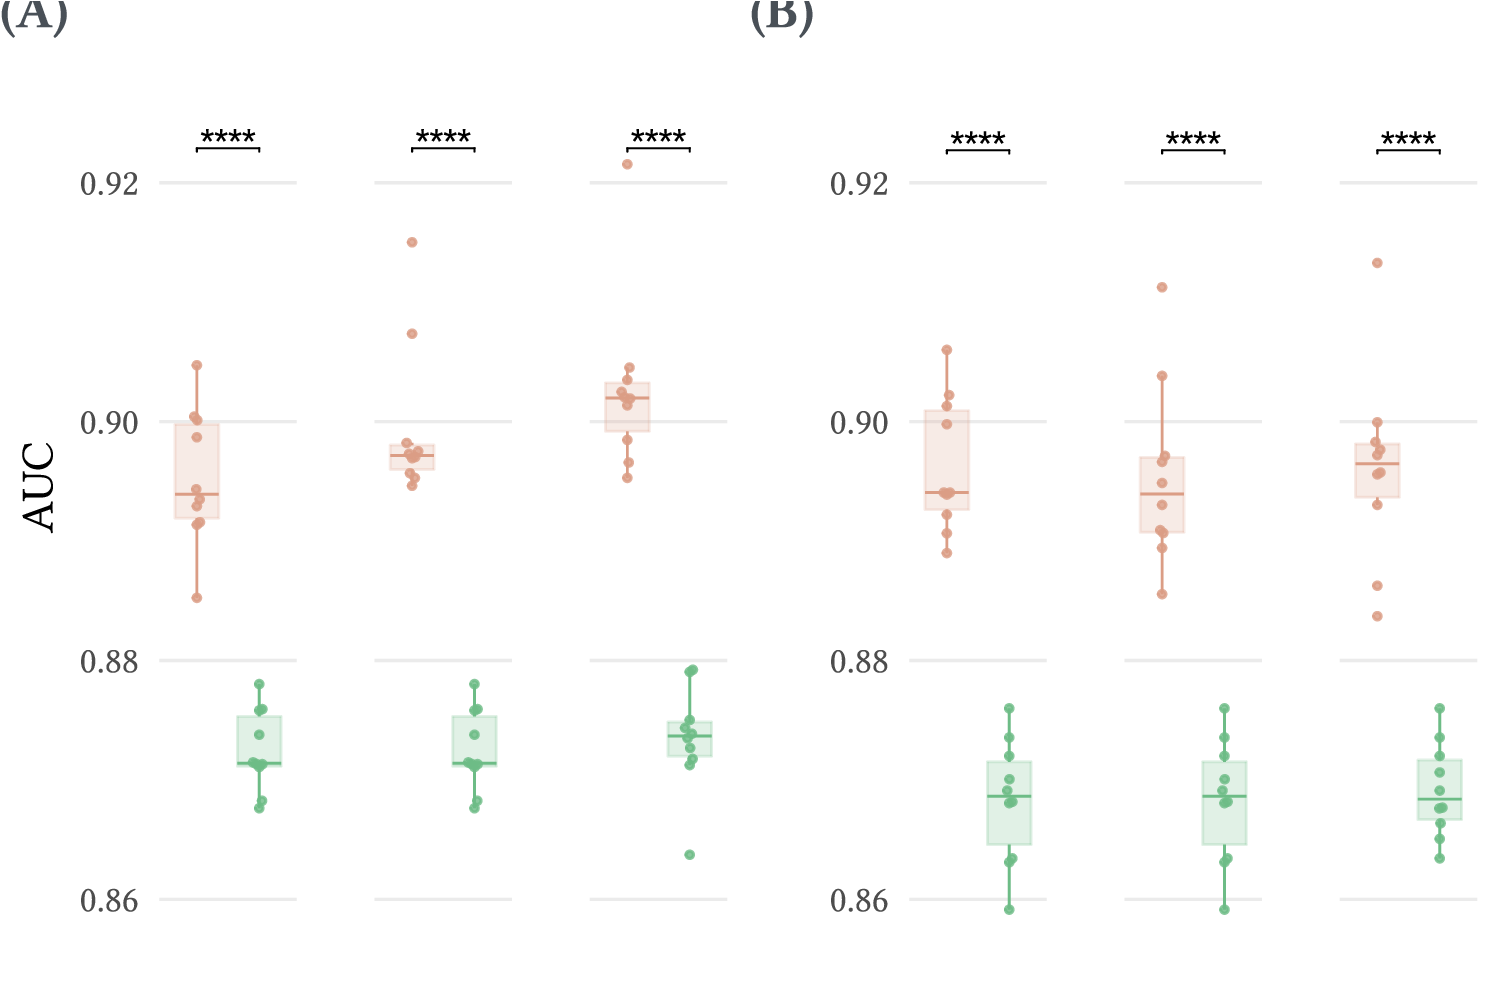
\includegraphics{figs/comparisonABCCMAES} 

}

\caption{Comparison of CMA-ES and ABC-rejection methods, with three occurrence subsets of beech, on \textbf{(A)} calibration AUC (only calibration points) and \textbf{(B)} total AUC (every presence/absence points). Each point is a calibration run. The black horizontal bars represent the pairwise Mann–Whitney tests between the two methods on the same subset. CMA-ES is red and ABC green.}\label{fig:comparisonABCCMAES}
\end{figure}

\hypertarget{discussion}{%
\section{3. Discussion}\label{discussion}}

\hypertarget{performance-and-advantages-of-cma-es-to-calibrate-complex-models-in-ecology}{%
\subsection{3.1. Performance and advantages of CMA-ES to calibrate
complex models in
ecology}\label{performance-and-advantages-of-cma-es-to-calibrate-complex-models-in-ecology}}

Our results are the first to demonstrate that inverse calibration with
CMA-ES is feasible and provide good results for complex and
runtime-expensive ecological models.\\
With a subsampling of species occurrence data, the algorithm succeeds in
finding parameter sets which provide high AUC values. The predictions of
the calibrated models are sharply improved compared to classical
(forward) parametrization (\hyperref[fig:phenofitmaps]{Figure 1} and
\hyperref[fig:castaneamaps]{Figure 2}). AUC values obtained using CMA-ES
were as good as the ones generally obtained with correlative models. Two
striking examples are the increase in the performance of PHENOFIT model
for silver fir, from 0.72 to 0.9, and of CASTANEA model for holm oak,
from 0.7 to 0.95. Moreover, CMA-ES performed equally well regardless of
the species occurrence subset used during calibration
(\hyperref[fig:cmaesrepAUCcal]{Figure 3.B.}), and thus permitted to find
a good compromise between computational cost and calibration efficiency.

CMA-ES is a ``generic'' optimizer which can be applied to various
problems. It is easy to use as it does not require an extensive tuning
to efficiently explore the parameter space. We only had to choose the
population size \(\lambda\), and the initial search region (initial
starting point and step size \(\sigma\)). As well as being quasi
parameter-free, CMA-ES has several structural advantages:\\
- the covariance matrix allows to learn second-order information
(pairwise dependencies between parameters)\\
- the covariance matrix adaptation is particularly efficient to deal
with ill-conditioned and non-separable problems
(\protect\hyperlink{ref-Hansen2011}{Hansen \emph{et al.} 2011})\\
- the update of the step size \(\sigma\) (i.e.~mutation force) prevents
premature convergence (\protect\hyperlink{ref-Hansen2001}{Hansen \&
Ostermeier 2001})\\
CMA-ES has been shown to outperform several other optimization
algorithms (\protect\hyperlink{ref-Hansen2010}{Hansen \emph{et al.}
2010}), and is usually the most efficient method when the target cost
(i.e.~the number of objective function evaluations) is about \(100*N\)
(\(N\) being the dimension of the parameter search space,
\protect\hyperlink{ref-Baeck2013}{Bäck \emph{et al.} 2013}). Here we
show that it outperforms the widely used ABC optimization method too.

\hypertarget{non-identifiability-of-parameter-values}{%
\subsection{3.2. Non-identifiability of parameter
values}\label{non-identifiability-of-parameter-values}}

There can be a strong dependence between process-based model
parameters.\\
In both models used in this study, biological mechanisms are explicitly
calculated in several submodels (e.g.~a leaf unfolding submodel or a
stomatal opening submodel). A submodel output has inevitably a
significant influence on the other submodels as biological processes can
be highly dependent with feedbacks: in CASTANEA, for example, the
stomatal opening affects the photosynthesis, and \emph{vice versa}.
Within each submodel, parameters are also strongly dependent because of
structural correlations. To illustrate this problem, we focused on beech
leaf unfolding submodel of PHENOFIT (see
\protect\hyperlink{appendixA}{Appendix A}). This model has 6 parameters
(\protect\hyperlink{ref-Chuine2000}{Chuine 2000}): a starting date of
the processes (\(t_0\)), one parameter describing the response function
to temperature during the dormancy phase (\(T_b\)), two parameters
describing the response function to temperature during the phase of bud
growth (\(d_T\), \(T_{50}\)), and two parameters representing the sums
of the daily responses to temperature during bud dormancy (\(C_{crit}\))
and during bud growth (\(F_{crit}\)) that respectively determine the
date of bud dormancy break and the date of leaf unfolding (see
\protect\hyperlink{appendixG}{Appendix G} for details). Since no
information on the date of bud dormancy break is available for the
calibration, a first structural negative correlation exists between
\(C_{crit}\) and \(F_{crit}\): the same leaf unfolding date can be
obtained with either a long dormancy phase and short bud growth phase or
a short dormancy phase and a long bud growth phase. Other structural
correlations exist between \(T_b\) and \(C_{crit}\) on the one hand and
\(d_T\)/\(T_{50}\) and \(F_{crit}\) on the other hand: for example, a
rapid accumulation of chilling units with a high critical chilling
requirement could yield identical results as a slow accumulation with a
low critical chilling requirement (i.e.~the threshold temperature
\(T_{b}\) and the critical chilling requirement \(C_{crit}\) are
dependent, see Figure G.1.A. in \protect\hyperlink{appendixG}{Appendix
G}).

Consequently, several parameter sets may be statistically equivalent and
parameters non-identifiable. In fact, calibration repetitions gave
diverging parameter values (\hyperref[fig:unfoldingplots]{Figure 4})
while being efficient in distinguishing between species presence and
absence (i.e.~AUC \textasciitilde{} 0.9,
\hyperref[fig:cmaesrepAUCcal]{Figure 3}). Thus, even if the calibrated
model describes the observed species distribution very well, it does not
necessarily mean that parameter values are ecologically relevant. This
concern is similar to the criticisms against correlative SDMs, in which
parameter values and correlations that well reproduce species ranges not
necessarily describe a complex biological reality. In our case, the
constraints imposed by the explicit mathematical equations embedded in
our models were not sufficient to ensure calibration convergence towards
similar solutions that would have suggested a high biological realism.
However, it is worth noting that we deliberately chose large parameter
ranges (although biologically realistic, i.e.~corresponding to the
observations made on the different processes modelled across different
species) in order to give free rein to the optimization algorithm. As
our goal was to assess the performance of CMA-ES objectively, we did not
attempt to minimize this non-identifiability issue by restrincting the
parameter space.

\hypertarget{methodological-issues-and-perspectives-of-our-study}{%
\subsection{3.3. Methodological issues and perspectives of our
study}\label{methodological-issues-and-perspectives-of-our-study}}

Our goal here was to investigate the performance of CMA-ES to calibrate
quite complex process-based species distribution models using species
occurrence data. We did not attempt to validate our parametrizations
using independent data, and AUC was only used to determine if model
outputs were consistent with species distributions. However, AUC is
scale-invariant (it measures how well predictions are ranked rather than
their absolute values), and prevents us from obtaining calibrated
outputs with more ecological meaning. For example, in PHENOFIT, one
species with a fitness of \(0.8\) could be considered as absent whereas
another one as present. Further work could thus be conducted to examine
the effects of choosing a different objective function.

We compared CMA-ES with a fairly simple but frequently used ABC
algorithm because it is widely recognized as an efficient method, and
has several advantages including its relative methodological simplicity
(which makes it quite easy to implement) and its ability to quantify the
uncertainty of the parameters. We did so to provide elements of
comparison in order to evaluate CMA-ES performance, and we did not aim
to argue for the merits of one approach over another. Higher
computational efficiency might be obtained using other types of ABC
algorithms, such as Sequential Monte Carlo
(\protect\hyperlink{ref-Beaumont2010}{Beaumont 2010}).

It would also be valuable to use a significantly higher computing power,
with an adapted version of CMA-ES. To improve the global search
performance of CMA-ES, we slightly increased the population size
\(\lambda\) (\protect\hyperlink{ref-Hansen2004}{Hansen \& Kern 2004})
and used a computing cluster to evaluate \(\lambda\) functions in
parallel. We were able to use between 40 and 120 cores, which is far
from the computing power of some GPUs (\textgreater{} 2000 cores). In
this case, choosing a very large population size might not be the best
choice. To use efficiently this large parallel computing power, one
could rather use a CMA-ES restart strategy (e.g.~IPOP-CMA-ES,
\protect\hyperlink{ref-Auger2005}{Auger \& Hansen 2005}), where
population size is successively increased (by a factor of 2), and run
these calibrations in parallel. Moreover, when a model requires a high
computation time and thus only a small budget can be afforded, the
original fitness function could be approximated with a surrogate model
in order to reduce the number of original function evaluations required
(e.g. \protect\hyperlink{ref-Auger2004}{Auger \emph{et al.} 2004} ;
\protect\hyperlink{ref-Loshchilov2013}{Loshchilov \emph{et al.} 2013}).

Finally, several authors advocate for process-based modeling approaches
relying upon species response functions that are a priori defined (e.g.
\protect\hyperlink{ref-Higgins2020}{Higgins \emph{et al.} 2020}).
However, the main limitation of such models is the data availability to
infer their parameters (\protect\hyperlink{ref-Urban2016}{Urban \emph{et
al.} 2016}). Forward parametrization is often long and arduous, and we
demonstrated that CMA-ES backward parametrization of PBMs can be a
powerful technique. One possible way to facilitate parameter values
estimation would be to use backward calibration. In particular, CMA-ES
driven by species occurrence data could be used to calibrate submodels
whose parameter values can hardly be experimentally measured. However,
when a structural correlation exists (as in the leaf unfolding
submodel), backward calibration might not provide the right parameter
estimates. In such a case, observations and measurements are necessary
to determine \emph{a posteriori} which estimates are the most realistic.
A combination of both forward and backward calibrations might offer a
new perspective for spreading the use of process-based models in
predictive ecology, especially for climate change impact studies.

\hypertarget{acknowledgements}{%
\section{Acknowledgements}\label{acknowledgements}}

The authors would like to thank Hendrik Davi for helping us in using the
CASTANEA model. We are also deeply grateful for many helpful comments
from Florence Tauc. Finally, we would like to thank François de Coligny,
manager of the CAPSIS platform, and the GenOuest and TGCC teams for
their support. V.V. was supported by a GAIA doctoral school PhD
Fellowship.

\hypertarget{conflict-of-interest}{%
\section{Conflict of interest}\label{conflict-of-interest}}

The authors have no conflicts of interest to declare.

\hypertarget{author-contributions}{%
\section{Author contributions}\label{author-contributions}}

I.C. devised the main conceptual ideas. V.V. worked out the technical
details, performed the numerical calculations and wrote the first draft
of the manuscript. The two authors discussed the analyses and the
results, and contributed to the final manuscript.

\hypertarget{data-availability}{%
\section{Data availability}\label{data-availability}}

ERA5-Land dataset is available on the
\href{https://cds.climate.copernicus.eu/cdsapp\#!/dataset/reanalysis-era5-land?tab=overview}{Copernicus
Climate Change Service website}. EU-SoilHydroGrids is available on the
\href{https://esdac.jrc.ec.europa.eu/content/3d-soil-hydraulic-database-europe-1-km-and-250-m-resolution}{European
Soil Data Centre website}. SoilGrids250m is available on the
\href{https://www.isric.org/explore/soilgrids}{International Soil
Reference and Information Centre website}. EU-Forest database is
available on
\href{https://figshare.com/collections/A_high-resolution_pan-European_tree_occurrence_dataset/3288407}{FigShare}.
The R code associated with this work will be made available on GitLab
upon acceptance of the manuscript.

\hypertarget{references}{%
\section{References}\label{references}}

\setlength{\parindent}{-0.2in}
\setlength{\leftskip}{0.2in}
\setlength{\parskip}{8pt}
\vspace*{-0.2in}

\noindent

\hypertarget{refs}{}
\begin{CSLReferences}{1}{0}
\leavevmode\vadjust pre{\hypertarget{ref-Araujo2019}{}}%
Araújo, M.B., Anderson, R.P., Márcia Barbosa, A., Beale, C.M., Dormann,
C.F., Early, R., Garcia, R.A., Guisan, A., Maiorano, L., Naimi, B.,
O'Hara, R.B., Zimmermann, N.E. \& Rahbek, C. (2019). Standards for
distribution models in biodiversity assessments. \emph{Science
Advances}, \textbf{5}.
\href{https://doi.org/10.1126/sciadv.aat4858}{10.1126/sciadv.aat4858}

\leavevmode\vadjust pre{\hypertarget{ref-Auger2005}{}}%
Auger, A. \& Hansen, N. (2005). A restart {CMA} evolution strategy with
increasing population size. \emph{2005 {IEEE} {Congress} on
{Evolutionary} {Computation}}, pp. 1769--1776 Vol. 2.

\leavevmode\vadjust pre{\hypertarget{ref-Auger2004}{}}%
Auger, A., Schoenauer, M. \& Vanhaecke, N. (2004). {LS}-{CMA}-{ES}: {A}
{Second}-{Order} {Algorithm} for {Covariance} {Matrix} {Adaptation}.
\emph{Parallel {Problem} {Solving} from {Nature} - {PPSN} {VIII}} (eds
X. Yao, E.K. Burke, J.A. Lozano, J. Smith, J.J. Merelo-Guervós, J.A.
Bullinaria, J.E. Rowe, P. Tino, A. Kabán \& H.-P. Schwefel), pp.
182--191. Lecture {Notes} in {Computer} {Science}. Springer, Berlin,
Heidelberg.

\leavevmode\vadjust pre{\hypertarget{ref-Baeck2013}{}}%
Bäck, T., Foussette, C. \& Krause, P. (2013). Empirical {Analysis}. (eds
T. Bäck, C. Foussette \& P. Krause), pp. 55--83. Natural {Computing}
{Series}. Springer, Berlin, Heidelberg.

\leavevmode\vadjust pre{\hypertarget{ref-Ballings2013}{}}%
Ballings, M. \& Van den Poel, D. (2013). \emph{AUC: Threshold
independent performance measures for probabilistic classifiers.}

\leavevmode\vadjust pre{\hypertarget{ref-Barnosky2012}{}}%
Barnosky, A.D., Hadly, E.A., Bascompte, J., Berlow, E.L., Brown, J.H.,
Fortelius, M., Getz, W.M., Harte, J., Hastings, A., Marquet, P.A.,
Martinez, N.D., Mooers, A., Roopnarine, P., Vermeij, G., Williams, J.W.,
Gillespie, R., Kitzes, J., Marshall, C., Matzke, N., Mindell, D.P.,
Revilla, E. \& Smith, A.B. (2012). Approaching a state shift in
{Earth}'s biosphere. \emph{Nature}, \textbf{486}, 52--58.
\href{https://doi.org/10.1038/nature11018}{10.1038/nature11018}

\leavevmode\vadjust pre{\hypertarget{ref-Beaumont2010}{}}%
Beaumont, M.A. (2010). Approximate {Bayesian} {Computation} in
{Evolution} and {Ecology}. \emph{Annual Review of Ecology, Evolution,
and Systematics}, \textbf{41}, 379--406.

\leavevmode\vadjust pre{\hypertarget{ref-Bengtsson2021}{}}%
Bengtsson, H. (2021). A unifying framework for parallel and distributed
processing in r using futures.

\leavevmode\vadjust pre{\hypertarget{ref-EVM2003}{}}%
Bohn, U., Neuhäusl, R., Gisela Gollub, Hettwer, C., Neuhäuslová, Z.,
Raus, T., Schlüter, H. \& Weber, H. (2003). \emph{Map of the natural
vegetation of europe - scale 1:2500000}.

\leavevmode\vadjust pre{\hypertarget{ref-Cai2019}{}}%
Cai, J. (2019). \emph{Humidity: Calculate water vapor measures from
temperature and dew point}.

\leavevmode\vadjust pre{\hypertarget{ref-Chuine2000}{}}%
Chuine, I. (2000). A {Unified} {Model} for {Budburst} of {Trees}.
\emph{Journal of Theoretical Biology}, \textbf{207}, 337--347.
\href{https://doi.org/10.1006/jtbi.2000.2178}{10.1006/jtbi.2000.2178}

\leavevmode\vadjust pre{\hypertarget{ref-Chuine2001}{}}%
Chuine, I. \& Beaubien, E.G. (2001). Phenology is a major determinant of
tree species range. \emph{Ecology Letters}, \textbf{4}, 500--510.
\href{https://doi.org/10.1046/j.1461-0248.2001.00261.x}{10.1046/j.1461-0248.2001.00261.x}

\leavevmode\vadjust pre{\hypertarget{ref-Collange2010}{}}%
Collange, G., Reynaud, S. \& Hansen, N. (2010). Covariance matrix
adaptation evolution strategy for multidisciplinary optimization of
expendable launcher family. \emph{13th AIAA/ISSMO multidisciplinary
analysis optimization conference}.

\leavevmode\vadjust pre{\hypertarget{ref-Connolly2017}{}}%
Connolly, S.R., Keith, S.A., Colwell, R.K. \& Rahbek, C. (2017).
Process, {Mechanism}, and {Modeling} in {Macroecology}. \emph{Trends in
Ecology \& Evolution}, \textbf{32}, 835--844.
\href{https://doi.org/10.1016/j.tree.2017.08.011}{10.1016/j.tree.2017.08.011}

\leavevmode\vadjust pre{\hypertarget{ref-Csillery2010}{}}%
Csilléry, K., Blum, M.G.B., Gaggiotti, O.E. \& François, O. (2010).
Approximate {Bayesian} {Computation} ({ABC}) in practice. \emph{Trends
in Ecology \& Evolution}, \textbf{25}, 410--418.
\href{https://doi.org/10.1016/j.tree.2010.04.001}{10.1016/j.tree.2010.04.001}

\leavevmode\vadjust pre{\hypertarget{ref-Davi2017}{}}%
Davi, H. \& Cailleret, M. (2017). Assessing drought-driven mortality
trees with physiological process-based models. \emph{Agricultural and
Forest Meteorology}, \textbf{232}, 279--290.
\href{https://doi.org/10.1016/j.agrformet.2016.08.019}{10.1016/j.agrformet.2016.08.019}

\leavevmode\vadjust pre{\hypertarget{ref-Davi2006}{}}%
Davi, H., Dufrêne, E., Francois, C., Le Maire, G., Loustau, D., Bosc,
A., Rambal, S., Granier, A. \& Moors, E. (2006). Sensitivity of water
and carbon fluxes to climate changes from 1960 to 2100 in {European}
forest ecosystems. \emph{Agricultural and Forest Meteorology},
\textbf{141}, 35--56.
\href{https://doi.org/10.1016/j.agrformet.2006.09.003}{10.1016/j.agrformet.2006.09.003}

\leavevmode\vadjust pre{\hypertarget{ref-Davi2005}{}}%
Davi, H., Dufrêne, E., Granier, A., Le Dantec, V., Barbaroux, C.,
François, C. \& Bréda, N. (2005). Modelling carbon and water cycles in a
beech forest: {Part} {II}.: {Validation} of the main processes from
organ to stand scale. \emph{Ecological Modelling}, \textbf{185},
387--405.
\href{https://doi.org/10.1016/j.ecolmodel.2005.01.003}{10.1016/j.ecolmodel.2005.01.003}

\leavevmode\vadjust pre{\hypertarget{ref-Delpierre2012}{}}%
Delpierre, N., Soudani, K., François, C., Le Maire, G., Bernhofer, C.,
Kutsch, W., Misson, L., Rambal, S., Vesala, T. \& Dufrêne, E. (2012).
Quantifying the influence of climate and biological drivers on the
interannual variability of carbon exchanges in {European} forests
through process-based modelling. \emph{Agricultural and Forest
Meteorology}, \textbf{154-155}, 99--112.
\href{https://doi.org/10.1016/j.agrformet.2011.10.010}{10.1016/j.agrformet.2011.10.010}

\leavevmode\vadjust pre{\hypertarget{ref-Dormann2012}{}}%
Dormann, C.F., Schymanski, S.J., Cabral, J., Chuine, I., Graham, C.,
Hartig, F., Kearney, M., Morin, X., Römermann, C., Schröder, B. \&
Singer, A. (2012). Correlation and process in species distribution
models: Bridging a dichotomy. \emph{Journal of Biogeography},
\textbf{39}, 2119--2131.
\href{https://doi.org/10.1111/j.1365-2699.2011.02659.x}{10.1111/j.1365-2699.2011.02659.x}

\leavevmode\vadjust pre{\hypertarget{ref-Dufrene2005}{}}%
Dufrêne, E., Davi, H., François, C., Maire, G. le, Dantec, V.L. \&
Granier, A. (2005). Modelling carbon and water cycles in a beech forest:
{Part} {I}: {Model} description and uncertainty analysis on modelled
{NEE}. \emph{Ecological Modelling}, \textbf{185}, 407--436.
\href{https://doi.org/10.1016/j.ecolmodel.2005.01.004}{10.1016/j.ecolmodel.2005.01.004}

\leavevmode\vadjust pre{\hypertarget{ref-Duputie2015}{}}%
Duputié, A., Rutschmann, A., Ronce, O. \& Chuine, I. (2015).
Phenological plasticity will not help all species adapt to climate
change. \emph{Global Change Biology}, \textbf{21}, 3062--3073.
\href{https://doi.org/10.1111/gcb.12914}{10.1111/gcb.12914}

\leavevmode\vadjust pre{\hypertarget{ref-Duputie2014}{}}%
Duputié, A., Zimmermann, N.E. \& Chuine, I. (2014). Where are the wild
things? Why we need better data on species distribution. \emph{Global
Ecology and Biogeography}, \textbf{23}, 457--467.
\href{https://doi.org/10.1111/geb.12118}{10.1111/geb.12118}

\leavevmode\vadjust pre{\hypertarget{ref-Evans2012}{}}%
Evans, M.R. (2012). Modelling ecological systems in a changing world.
\emph{Philosophical Transactions of the Royal Society B: Biological
Sciences}, \textbf{367}, 181--190.
\href{https://doi.org/10.1098/rstb.2011.0172}{10.1098/rstb.2011.0172}

\leavevmode\vadjust pre{\hypertarget{ref-Fitzpatrick2018}{}}%
Fitzpatrick, M.C., Blois, J.L., Williams, J.W., Nieto-Lugilde, D.,
Maguire, K.C. \& Lorenz, D.J. (2018). How will climate novelty influence
ecological forecasts? {Using} the {Quaternary} to assess future
reliability. \emph{Global Change Biology}, \textbf{24}, 3575--3586.
\href{https://doi.org/10.1111/gcb.14138}{10.1111/gcb.14138}

\leavevmode\vadjust pre{\hypertarget{ref-Fourcade2018}{}}%
Fourcade, Y., Besnard, A.G. \& Secondi, J. (2018). Paintings predict the
distribution of species, or the challenge of selecting environmental
predictors and evaluation statistics. \emph{Global Ecology and
Biogeography}, \textbf{27}, 245--256.
\href{https://doi.org/10.1111/geb.12684}{10.1111/geb.12684}

\leavevmode\vadjust pre{\hypertarget{ref-Gagne2008}{}}%
Gagné, C., Beaulieu, J., Parizeau, M. \& Thibault, S. (2008).
Human-competitive lens system design with evolution strategies.
\emph{Applied Soft Computing}, \textbf{8}, 1439--1452.
\href{https://doi.org/10.1016/j.asoc.2007.10.018}{10.1016/j.asoc.2007.10.018}

\leavevmode\vadjust pre{\hypertarget{ref-Gardner2020}{}}%
Gardner, E., Breeze, T.D., Clough, Y., Smith, H.G., Baldock, K.C.R.,
Campbell, A., Garratt, M.P.D., Gillespie, M.A.K., Kunin, W.E.,
McKerchar, M., Memmott, J., Potts, S.G., Senapathi, D., Stone, G.N.,
Wäckers, F., Westbury, D.B., Wilby, A. \& Oliver, T.H. (2020). Reliably
predicting pollinator abundance: {Challenges} of calibrating
process-based ecological models. \emph{Methods in Ecology and
Evolution}, \textbf{11}, 1673--1689.
\href{https://doi.org/10.1111/2041-210X.13483}{10.1111/2041-210X.13483}

\leavevmode\vadjust pre{\hypertarget{ref-Gauzere2020}{}}%
Gauzere, J., Teuf, B., Davi, H., Chevin, L.-M., Caignard, T., Leys, B.,
Delzon, S., Ronce, O. \& Chuine, I. (2020). Where is the optimum?
{Predicting} the variation of selection along climatic gradients and the
adaptive value of plasticity. {A} case study on tree phenology.
\emph{Evolution Letters}, \textbf{4}, 109--123.
\href{https://doi.org/10.1002/evl3.160}{10.1002/evl3.160}

\leavevmode\vadjust pre{\hypertarget{ref-GBIF2022}{}}%
GBIF. (2022). The global biodiversity information facility.
\url{https://www.gbif.org} {[}accessed 24 January 2022{]}

\leavevmode\vadjust pre{\hypertarget{ref-Guisan2005}{}}%
Guisan, A. \& Thuiller, W. (2005). Predicting species distribution:
Offering more than simple habitat models. \emph{Ecology Letters},
\textbf{8}, 993--1009.
\href{https://doi.org/10.1111/j.1461-0248.2005.00792.x}{10.1111/j.1461-0248.2005.00792.x}

\leavevmode\vadjust pre{\hypertarget{ref-Guo2016}{}}%
Guo, D., Westra, S. \& Maier, H.R. (2016). An {R} package for modelling
actual, potential and reference evapotranspiration. \emph{Environmental
Modelling \& Software}, \textbf{78}, 216--224.
\href{https://doi.org/10.1016/j.envsoft.2015.12.019}{10.1016/j.envsoft.2015.12.019}

\leavevmode\vadjust pre{\hypertarget{ref-Hansen2016}{}}%
Hansen, N. (2016). The CMA evolution strategy: A tutorial.

\leavevmode\vadjust pre{\hypertarget{ref-Hansen2006}{}}%
Hansen, N. (2006). The {CMA} {Evolution} {Strategy}: {A} {Comparing}
{Review}. (eds J.A. Lozano, P. Larrañaga, I. Inza \& E. Bengoetxea), pp.
75--102. Studies in {Fuzziness} and {Soft} {Computing}. Springer,
Berlin, Heidelberg.

\leavevmode\vadjust pre{\hypertarget{ref-Hansen2010}{}}%
Hansen, N., Auger, A., Ros, R., Finck, S. \& Posik, P. (2010).
{Comparing Results of 31 Algorithms from the Black-Box Optimization
Benchmarking BBOB-2009}. \emph{{ACM-GECCO Genetic and Evolutionary
Computation Conference}}. Portland, United States.

\leavevmode\vadjust pre{\hypertarget{ref-Hansen2004}{}}%
Hansen, N. \& Kern, S. (2004). Evaluating the {CMA} {Evolution}
{Strategy} on {Multimodal} {Test} {Functions}. \emph{Parallel {Problem}
{Solving} from {Nature} - {PPSN} {VIII}} (eds X. Yao, E.K. Burke, J.A.
Lozano, J. Smith, J.J. Merelo-Guervós, J.A. Bullinaria, J.E. Rowe, P.
Tino, A. Kabán \& H.-P. Schwefel), pp. 282--291. Lecture {Notes} in
{Computer} {Science}. Springer, Berlin, Heidelberg.

\leavevmode\vadjust pre{\hypertarget{ref-Hansen2009}{}}%
Hansen, N., Niederberger, A.S.P., Guzzella, L. \& Koumoutsakos, P.
(2009). A {Method} for {Handling} {Uncertainty} in {Evolutionary}
{Optimization} {With} an {Application} to {Feedback} {Control} of
{Combustion}. \emph{IEEE Transactions on Evolutionary Computation},
\textbf{13}, 180--197.
\href{https://doi.org/10.1109/TEVC.2008.924423}{10.1109/TEVC.2008.924423}

\leavevmode\vadjust pre{\hypertarget{ref-Hansen1996}{}}%
Hansen, N. \& Ostermeier, A. (1996). Adapting arbitrary normal mutation
distributions in evolution strategies: The covariance matrix adaptation.
\emph{Proceedings of {IEEE} {International} {Conference} on
{Evolutionary} {Computation}}, pp. 312--317.

\leavevmode\vadjust pre{\hypertarget{ref-Hansen2001}{}}%
Hansen, N. \& Ostermeier, A. (2001). Completely {Derandomized}
{Self}-{Adaptation} in {Evolution} {Strategies}. \emph{Evolutionary
Computation}, \textbf{9}, 159--195.
\href{https://doi.org/10.1162/106365601750190398}{10.1162/106365601750190398}

\leavevmode\vadjust pre{\hypertarget{ref-Hansen2011}{}}%
Hansen, N., Ros, R., Mauny, N., Schoenauer, M. \& Auger, A. (2011).
Impacts of invariance in search: {When} {CMA}-{ES} and {PSO} face
ill-conditioned and non-separable problems. \emph{Applied Soft
Computing}, \textbf{11}, 5755--5769.
\href{https://doi.org/10.1016/j.asoc.2011.03.001}{10.1016/j.asoc.2011.03.001}

\leavevmode\vadjust pre{\hypertarget{ref-Hartig2014}{}}%
Hartig, F., Dislich, C., Wiegand, T. \& Huth, A. (2014). Technical
{Note}: {Approximate} {Bayesian} parameterization of a process-based
tropical forest model. \emph{Biogeosciences}, \textbf{11}, 1261--1272.
\href{https://doi.org/10.5194/bg-11-1261-2014}{10.5194/bg-11-1261-2014}

\leavevmode\vadjust pre{\hypertarget{ref-Hengl2017}{}}%
Hengl, T., Jesus, J.M. de, Heuvelink, G.B.M., Gonzalez, M.R., Kilibarda,
M., Blagotic, A., Shangguan, W., Wright, M.N., Geng, X.,
Bauer-Marschallinger, B., Guevara, M.A., Vargas, R., MacMillan, R.A.,
Batjes, N.H., Leenaars, J.G.B., Ribeiro, E., Wheeler, I., Mantel, S. \&
Kempen, B. (2017). {SoilGrids250m}: {Global} gridded soil information
based on machine learning. \emph{PLOS ONE}, \textbf{12}, e0169748.
\href{https://doi.org/10.1371/journal.pone.0169748}{10.1371/journal.pone.0169748}

\leavevmode\vadjust pre{\hypertarget{ref-Higgins2020}{}}%
Higgins, S.I., Larcombe, M.J., Beeton, N.J., Conradi, T. \& Nottebrock,
H. (2020). Predictive ability of a process-based versus a correlative
species distribution model. \emph{Ecology and Evolution}, \textbf{10},
11043--11054.
\href{https://doi.org/10.1002/ece3.6712}{10.1002/ece3.6712}

\leavevmode\vadjust pre{\hypertarget{ref-Higgins2012}{}}%
Higgins, S.I., O'Hara, R.B. \& Römermann, C. (2012). A niche for biology
in species distribution models. \emph{Journal of Biogeography},
\textbf{39}, 2091--2095.
\href{https://doi.org/10.1111/jbi.12029}{10.1111/jbi.12029}

\leavevmode\vadjust pre{\hypertarget{ref-Hijmans2021}{}}%
Hijmans, R.J., Phillips, S., Leathwick, J. \& Elith, J. (2021).
\emph{Dismo: Species distribution modeling}.

\leavevmode\vadjust pre{\hypertarget{ref-Hill2020}{}}%
Hill, A., Laneurit, J., Lenain, R. \& Lucet, E. (2020). {Online gain
setting method for path tracking using CMA-ES: Application to off-road
mobile robot control}. \emph{{IROS 2020, International Conference on
Intelligent Robots and Systems}}. Las Vegas, United States.

\leavevmode\vadjust pre{\hypertarget{ref-AFE2005}{}}%
Jalas, J. \& Suominen, J. (1972--2005). \emph{Atlas florae europaeae}.
Committee for Mapping the Flora of Europe; Societas Biologica Fennica
Vanamo, Helsinki, Finland.

\leavevmode\vadjust pre{\hypertarget{ref-Journe2020}{}}%
Journé, V., Barnagaud, J., Bernard, C., Crochet, P. \& Morin, X. (2020).
Correlative climatic niche models predict real and virtual species
distributions equally well. \emph{Ecology}, \textbf{101}.
\href{https://doi.org/10.1002/ecy.2912}{10.1002/ecy.2912}

\leavevmode\vadjust pre{\hypertarget{ref-Kleidon2000}{}}%
Kleidon, A. \& Mooney, H.A. (2000). A global distribution of
biodiversity inferred from climatic constraints: Results from a
process-based modelling study. \emph{Global Change Biology}, \textbf{6},
507--523.
\href{https://doi.org/10.1046/j.1365-2486.2000.00332.x}{10.1046/j.1365-2486.2000.00332.x}

\leavevmode\vadjust pre{\hypertarget{ref-Lagarrigues2015}{}}%
Lagarrigues, G., Jabot, F., Lafond, V. \& Courbaud, B. (2015).
Approximate {Bayesian} computation to recalibrate individual-based
models with population data: {Illustration} with a forest simulation
model. \emph{Ecological Modelling}, \textbf{306}, 278--286.
\href{https://doi.org/10.1016/j.ecolmodel.2014.09.023}{10.1016/j.ecolmodel.2014.09.023}

\leavevmode\vadjust pre{\hypertarget{ref-Lenton2008}{}}%
Lenton, T.M., Held, H., Kriegler, E., Hall, J.W., Lucht, W., Rahmstorf,
S. \& Schellnhuber, H.J. (2008). Tipping elements in the {Earth}'s
climate system. \emph{Proceedings of the National Academy of Sciences},
\textbf{105}, 1786--1793.
\href{https://doi.org/10.1073/pnas.0705414105}{10.1073/pnas.0705414105}

\leavevmode\vadjust pre{\hypertarget{ref-Leroy2018}{}}%
Leroy, B., Delsol, R., Hugueny, B., Meynard, C.N., Barhoumi, C.,
Barbet-Massin, M. \& Bellard, C. (2018). Without quality
presence--absence data, discrimination metrics such as {TSS} can be
misleading measures of model performance. \emph{Journal of
Biogeography}, \textbf{45}, 1994--2002.
\href{https://doi.org/10.1111/jbi.13402}{10.1111/jbi.13402}

\leavevmode\vadjust pre{\hypertarget{ref-Lobo2008}{}}%
Lobo, J.M., Jiménez-Valverde, A. \& Real, R. (2008). {AUC}: A misleading
measure of the performance of predictive distribution models.
\emph{Global Ecology and Biogeography}, \textbf{17}, 145--151.
\href{https://doi.org/10.1111/j.1466-8238.2007.00358.x}{10.1111/j.1466-8238.2007.00358.x}

\leavevmode\vadjust pre{\hypertarget{ref-Loshchilov2013}{}}%
Loshchilov, I., Schoenauer, M. \& Sèbag, M. (2013). Bi-population
{CMA}-{ES} agorithms with surrogate models and line searches.
\emph{Proceedings of the 15th annual conference companion on {Genetic}
and evolutionary computation}, pp. 1177--1184. {GECCO} '13 {Companion}.
Association for Computing Machinery, New York, NY, USA.

\leavevmode\vadjust pre{\hypertarget{ref-Mauri2017}{}}%
Mauri, A., Strona, G. \& San-Miguel-Ayanz, J. (2017). {EU}-{Forest}, a
high-resolution tree occurrence dataset for {Europe}. \emph{Scientific
Data}, \textbf{4}, 160123.
\href{https://doi.org/10.1038/sdata.2016.123}{10.1038/sdata.2016.123}

\leavevmode\vadjust pre{\hypertarget{ref-Merow2014}{}}%
Merow, C., Smith, M.J., Edwards, T.C., Guisan, A., McMahon, S.M.,
Normand, S., Thuiller, W., Wüest, R.O., Zimmermann, N.E. \& Elith, J.
(2014). What do we gain from simplicity versus complexity in species
distribution models? \emph{Ecography}, \textbf{37}, 1267--1281.
\href{https://doi.org/10.1111/ecog.00845}{10.1111/ecog.00845}

\leavevmode\vadjust pre{\hypertarget{ref-Monnet2021}{}}%
Monnet, A.-C., Cilleros, K., Médail, F., Albassatneh, M.C., Arroyo, J.,
Bacchetta, G., Bagnoli, F., Barina, Z., Cartereau, M., Casajus, N.,
Dimopoulos, P., Domina, G., Doxa, A., Escudero, M., Fady, B., Hampe, A.,
Matevski, V., Misfud, S., Nikolic, T., Pavon, D., Roig, A., Barea, E.S.,
Spanu, I., Strid, A., Vendramin, G.G. \& Leriche, A. (2021). {WOODIV}, a
database of occurrences, functional traits, and phylogenetic data for
all {Euro}-{Mediterranean} trees. \emph{Scientific Data}, \textbf{8},
89.
\href{https://doi.org/10.1038/s41597-021-00873-3}{10.1038/s41597-021-00873-3}

\leavevmode\vadjust pre{\hypertarget{ref-Morin2007}{}}%
Morin, X., Augspurger, C. \& Chuine, I. (2007). Process-{Based}
{Modeling} of {Species}' {Distributions}: {What} {Limits} {Temperate}
{Tree} {Species}' {Range} {Boundaries}? \emph{Ecology}, \textbf{88},
2280--2291. \href{https://doi.org/10.1890/06-1591.1}{10.1890/06-1591.1}

\leavevmode\vadjust pre{\hypertarget{ref-Mouquet2015}{}}%
Mouquet, N., Lagadeuc, Y., Devictor, V., Doyen, L., Duputié, A.,
Eveillard, D., Faure, D., Garnier, E., Gimenez, O., Huneman, P., Jabot,
F., Jarne, P., Joly, D., Julliard, R., Kéfi, S., Kergoat, G.J., Lavorel,
S., Le Gall, L., Meslin, L., Morand, S., Morin, X., Morlon, H., Pinay,
G., Pradel, R., Schurr, F.M., Thuiller, W. \& Loreau, M. (2015).
{REVIEW}: {Predictive} ecology in a changing world. \emph{Journal of
Applied Ecology}, \textbf{52}, 1293--1310.
\href{https://doi.org/10.1111/1365-2664.12482}{10.1111/1365-2664.12482}

\leavevmode\vadjust pre{\hypertarget{ref-Sabater2021}{}}%
Muñoz Sabater, J. (2021). ERA5-land hourly data from 1950 to 1980.
\url{https://cds.climate.copernicus.eu/cdsapp\#!/dataset/reanalysis-era5-land}

\leavevmode\vadjust pre{\hypertarget{ref-Sabater2019}{}}%
Muñoz Sabater, J. (2019). ERA5-land hourly data from 1981 to present.
\url{https://cds.climate.copernicus.eu/cdsapp\#!/dataset/reanalysis-era5-land}

\leavevmode\vadjust pre{\hypertarget{ref-Pearman2008}{}}%
Pearman, P.B., Guisan, A., Broennimann, O. \& Randin, C.F. (2008). Niche
dynamics in space and time. \emph{Trends in Ecology \& Evolution},
\textbf{23}, 149--158.
\href{https://doi.org/10.1016/j.tree.2007.11.005}{10.1016/j.tree.2007.11.005}

\leavevmode\vadjust pre{\hypertarget{ref-Radeloff2015}{}}%
Radeloff, V.C., Williams, J.W., Bateman, B.L., Burke, K.D., Carter,
S.K., Childress, E.S., Cromwell, K.J., Gratton, C., Hasley, A.O.,
Kraemer, B.M., Latzka, A.W., Marin-Spiotta, E., Meine, C.D., Munoz,
S.E., Neeson, T.M., Pidgeon, A.M., Rissman, A.R., Rivera, R.J.,
Szymanski, L.M. \& Usinowicz, J. (2015). The rise of novelty in
ecosystems. \emph{Ecological Applications}, \textbf{25}, 2051--2068.
\href{https://doi.org/10.1890/14-1781.1}{10.1890/14-1781.1}

\leavevmode\vadjust pre{\hypertarget{ref-Saltre2013}{}}%
Saltré, F., Saint-Amant, R., Gritti, E.S., Brewer, S., Gaucherel, C.,
Davis, B.A.S. \& Chuine, I. (2013). Climate or migration: What limited
{European} beech post-glacial colonization? \emph{Global Ecology and
Biogeography}, \textbf{22}, 1217--1227.
\href{https://doi.org/10.1111/geb.12085}{10.1111/geb.12085}

\leavevmode\vadjust pre{\hypertarget{ref-Santini2021}{}}%
Santini, L., Benítez-López, A., Maiorano, L., Cengic, M. \& Huijbregts,
M.A.J. (2021). Assessing the reliability of species distribution
projections in climate change research. \emph{Diversity and
Distributions}, \textbf{27}, 1035--1050.
\href{https://doi.org/10.1111/ddi.13252}{10.1111/ddi.13252}

\leavevmode\vadjust pre{\hypertarget{ref-Singer2016}{}}%
Singer, A., Johst, K., Banitz, T., Fowler, M.S., Groeneveld, J.,
Gutiérrez, A.G., Hartig, F., Krug, R.M., Liess, M., Matlack, G., Meyer,
K.M., Pe'er, G., Radchuk, V., Voinopol-Sassu, A.-J. \& Travis, J.M.J.
(2016). Community dynamics under environmental change: {How} can next
generation mechanistic models improve projections of species
distributions? \emph{Ecological Modelling}, \textbf{326}, 63--74.
\href{https://doi.org/10.1016/j.ecolmodel.2015.11.007}{10.1016/j.ecolmodel.2015.11.007}

\leavevmode\vadjust pre{\hypertarget{ref-Steffen2018}{}}%
Steffen, W., Rockström, J., Richardson, K., Lenton, T.M., Folke, C.,
Liverman, D., Summerhayes, C.P., Barnosky, A.D., Cornell, S.E.,
Crucifix, M., Donges, J.F., Fetzer, I., Lade, S.J., Scheffer, M.,
Winkelmann, R. \& Schellnhuber, H.J. (2018). Trajectories of the {Earth}
{System} in the {Anthropocene}. \emph{Proceedings of the National
Academy of Sciences}, \textbf{115}, 8252--8259.
\href{https://doi.org/10.1073/pnas.1810141115}{10.1073/pnas.1810141115}

\leavevmode\vadjust pre{\hypertarget{ref-Toth2017}{}}%
Tóth, B., Weynants, M., Pásztor, L. \& Hengl, T. (2017). {3D} soil
hydraulic database of {Europe} at 250 m resolution. \emph{Hydrological
Processes}, \textbf{31}, 2662--2666.
\href{https://doi.org/10.1002/hyp.11203}{10.1002/hyp.11203}

\leavevmode\vadjust pre{\hypertarget{ref-Trautmann2011}{}}%
Trautmann, H., Mersmann, O. \& Arnu, D. (2011). \emph{Cmaes: Covariance
matrix adapting evolutionary strategy}.

\leavevmode\vadjust pre{\hypertarget{ref-Urban2015}{}}%
Urban, M.C. (2015). Accelerating extinction risk from climate change.
\emph{Science}, \textbf{348}, 571--573.
\href{https://doi.org/10.1126/science.aaa4984}{10.1126/science.aaa4984}

\leavevmode\vadjust pre{\hypertarget{ref-Urban2016}{}}%
Urban, M.C., Bocedi, G., Hendry, A.P., Mihoub, J.-B., Pe'er, G., Singer,
A., Bridle, J.R., Crozier, L.G., De Meester, L., Godsoe, W., Gonzalez,
A., Hellmann, J.J., Holt, R.D., Huth, A., Johst, K., Krug, C.B.,
Leadley, P.W., Palmer, S.C.F., Pantel, J.H., Schmitz, A., Zollner, P.A.
\& Travis, J.M.J. (2016). Improving the forecast for biodiversity under
climate change. \emph{Science}, \textbf{353}, aad8466.
\href{https://doi.org/10.1126/science.aad8466}{10.1126/science.aad8466}

\leavevmode\vadjust pre{\hypertarget{ref-Vaart2015}{}}%
Vaart, E. van der, Beaumont, M.A., Johnston, A.S.A. \& Sibly, R.M.
(2015). Calibration and evaluation of individual-based models using
{Approximate} {Bayesian} {Computation}. \emph{Ecological Modelling},
\textbf{312}, 182--190.
\href{https://doi.org/10.1016/j.ecolmodel.2015.05.020}{10.1016/j.ecolmodel.2015.05.020}

\leavevmode\vadjust pre{\hypertarget{ref-Warren2021}{}}%
Warren, D.L., Dornburg, A., Zapfe, K. \& Iglesias, T.L. (2021). The
effects of climate change on {Australia}'s only endemic {Pokémon}:
{Measuring} bias in species distribution models. \emph{Methods in
Ecology and Evolution}, \textbf{12}, 985--995.
\href{https://doi.org/10.1111/2041-210X.13591}{10.1111/2041-210X.13591}

\leavevmode\vadjust pre{\hypertarget{ref-Williams2007}{}}%
Williams, J.W., Jackson, S.T. \& Kutzbach, J.E. (2007). Projected
distributions of novel and disappearing climates by 2100 {AD}.
\emph{Proceedings of the National Academy of Sciences}, \textbf{104},
5738--5742.
\href{https://doi.org/10.1073/pnas.0606292104}{10.1073/pnas.0606292104}

\leavevmode\vadjust pre{\hypertarget{ref-Zurell2016}{}}%
Zurell, D., Thuiller, W., Pagel, J., Cabral, J.S., Münkemüller, T.,
Gravel, D., Dullinger, S., Normand, S., Schiffers, K.H., Moore, K.A. \&
Zimmermann, N.E. (2016). Benchmarking novel approaches for modelling
species range dynamics. \emph{Global Change Biology}, \textbf{22},
2651--2664. \href{https://doi.org/10.1111/gcb.13251}{10.1111/gcb.13251}

\end{CSLReferences}

\newpage

\hypertarget{appendixA}{%
\section{Supplementary Appendix A: Insights on the
models}\label{appendixA}}

\renewcommand*\thetable{A.\arabic{table}}
\renewcommand*\thefigure{A.\arabic{figure}}

\setcounter{figure}{0}
\setcounter{table}{0}

\pagenumbering{arabic}
\renewcommand*{\thepage}{A--\arabic{page}}

\begin{figure}[htbp]

{\centering 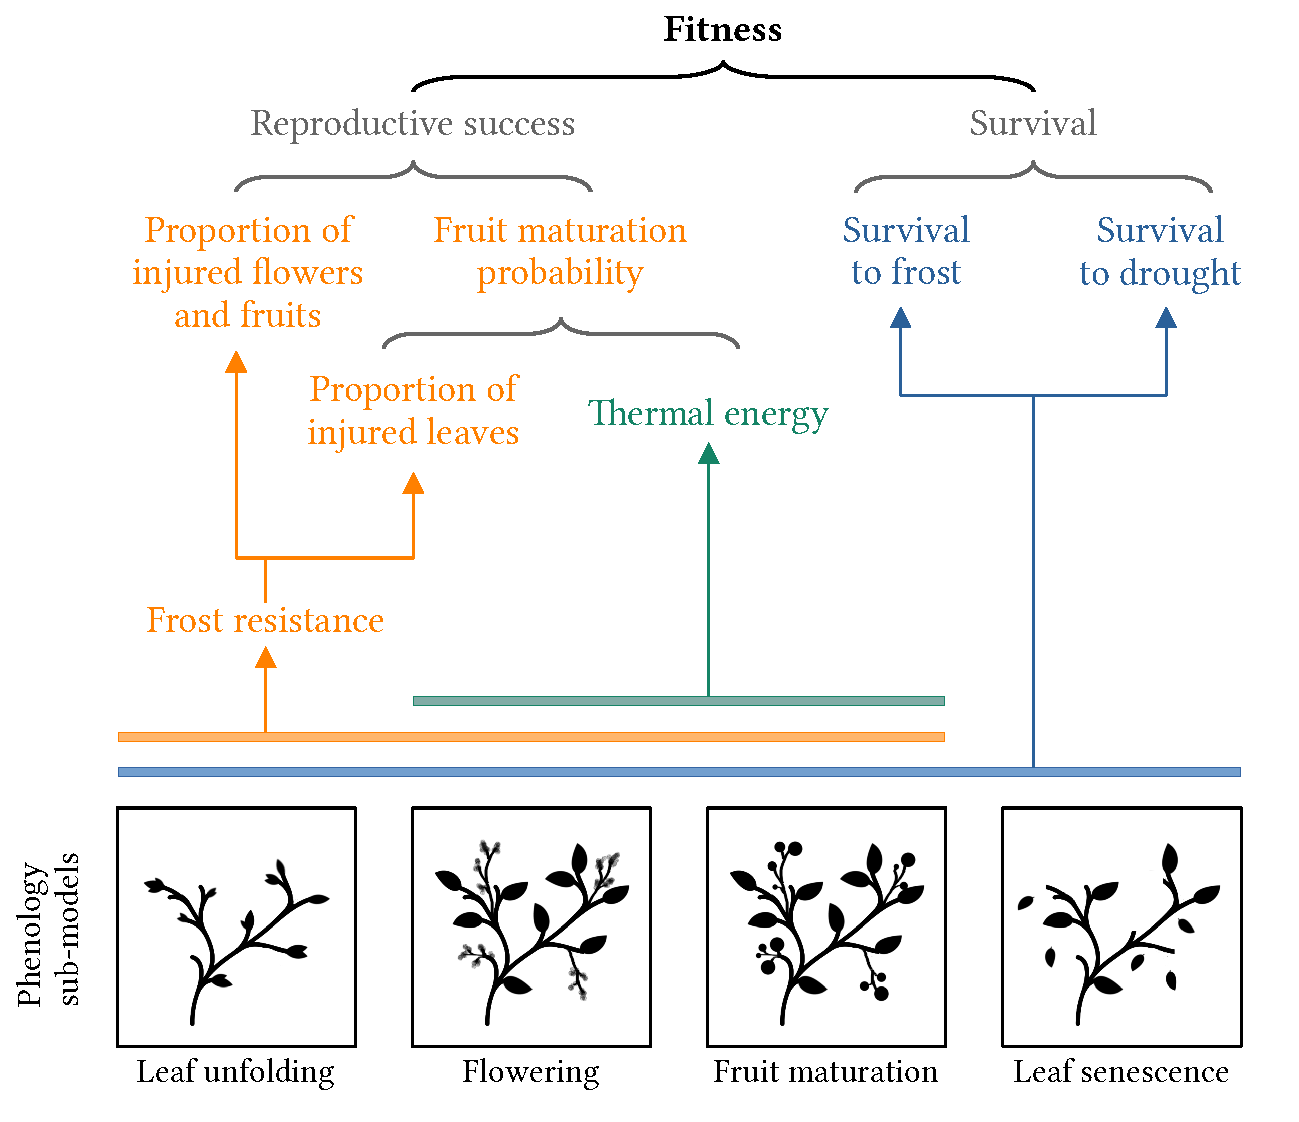
\includegraphics{figs/files/phenofit} 

}

\caption{PHENOFIT model in a nutshell.}\label{fig:phenofit_model}
\end{figure}

\begin{figure}[htbp]

{\centering 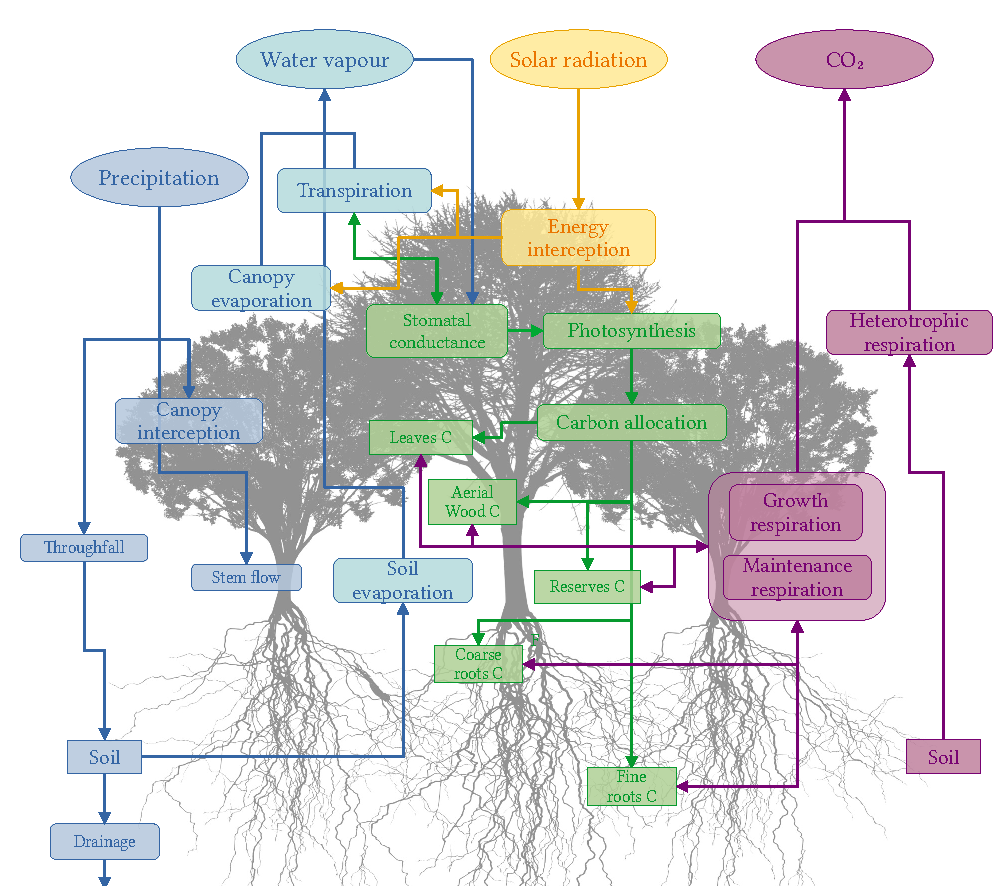
\includegraphics{figs/files/castanea_schema} 

}

\caption{CASTANEA model in a nutshell.}\label{fig:phenofit_model}
\end{figure}

\newpage

\hypertarget{appendixB}{%
\section{Supplementary Appendix B: Processing of occurrence
data}\label{appendixB}}

\renewcommand*\thetable{B.\arabic{table}}
\renewcommand*\thefigure{B.\arabic{figure}}

\setcounter{figure}{0}
\setcounter{table}{0}

\pagenumbering{arabic}
\renewcommand*{\thepage}{B--\arabic{page}}

\hfill \break

\begin{table}[!h]

\caption{\label{tab:unnamed-chunk-1}GBIF download links}
\centering
\begin{tabular}[t]{ccc}
\toprule
Species & Number of occurrences & Download link\\
\midrule
Fagus sylvatica & 718.898 & https://doi.org/10.15468/dl.e9wasa\\
Quercus ilex & 78.979 & https://doi.org/10.15468/dl.2a4haw\\
Abies alba & 119.891 & https://doi.org/10.15468/dl.my6c9t\\
\bottomrule
\end{tabular}
\end{table}

\hfill \break

\begin{figure}[htbp]

{\centering 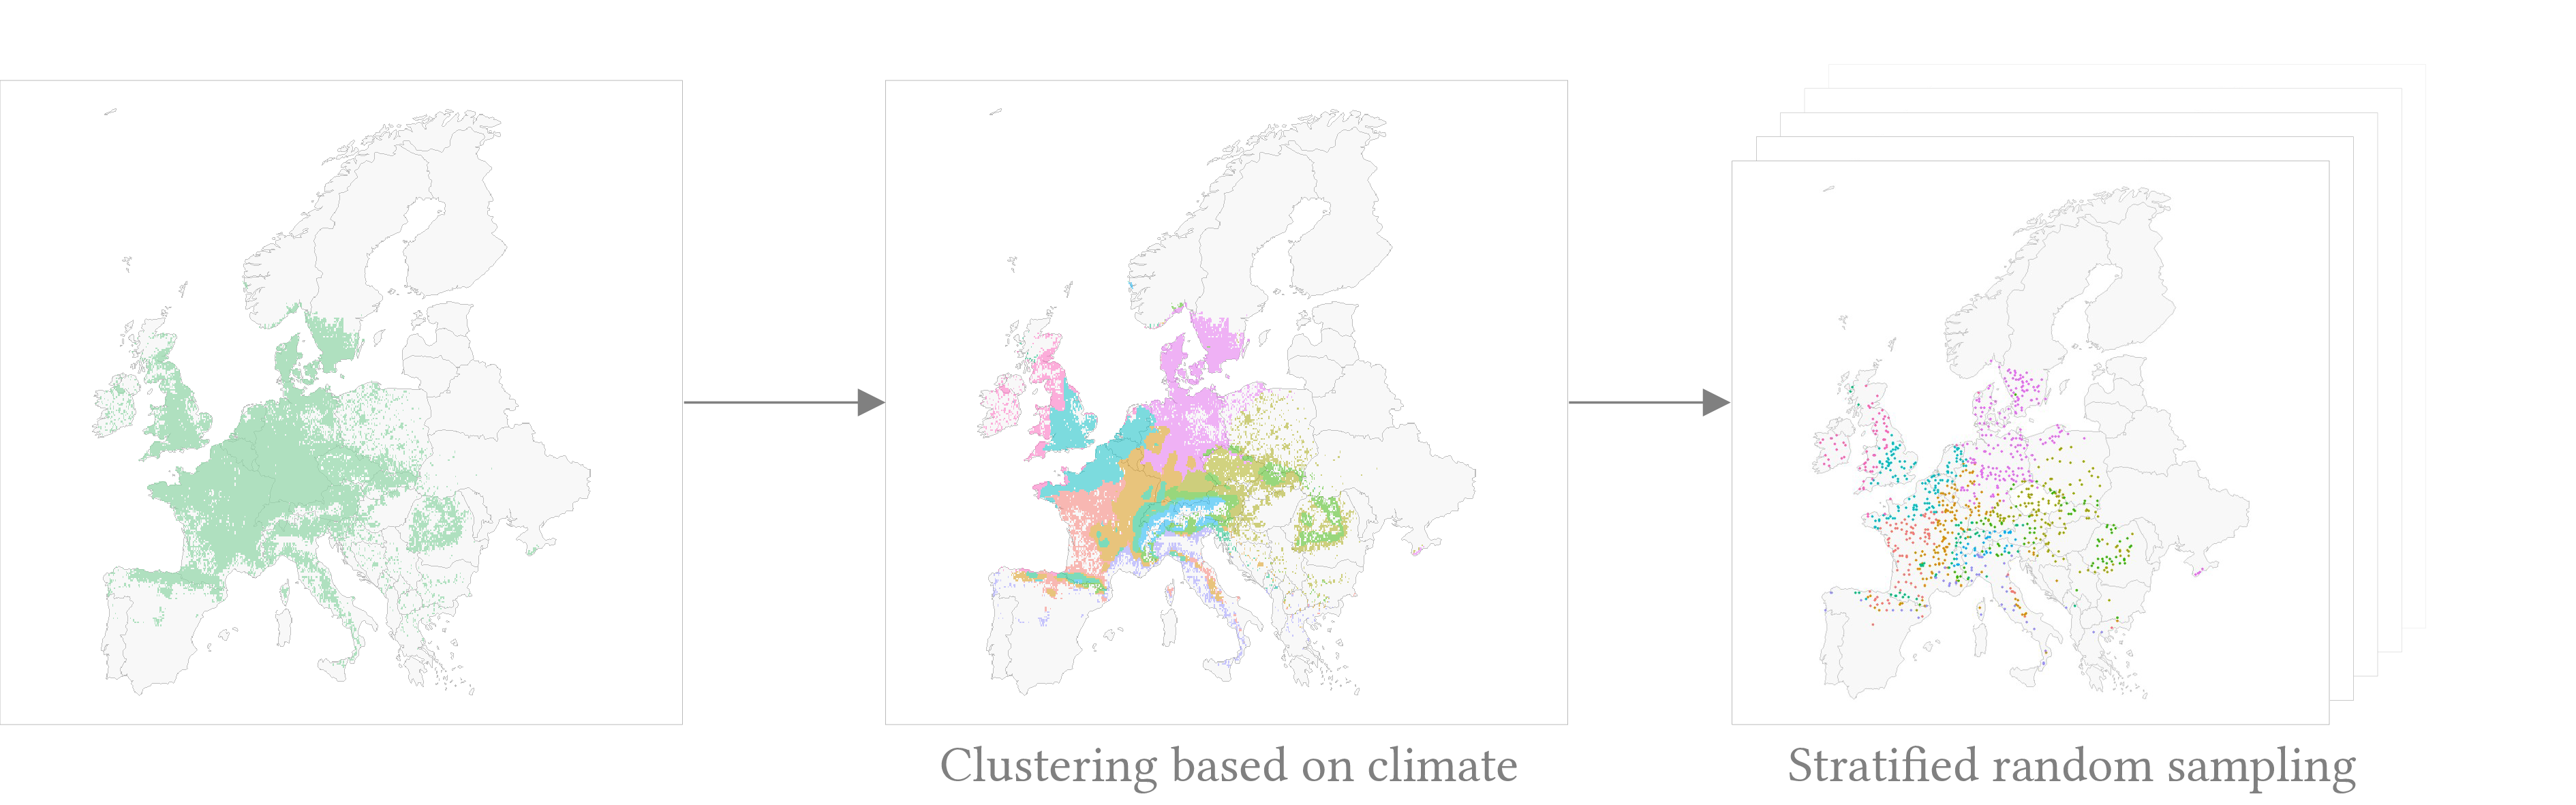
\includegraphics{figs/files/presence_clustering} 

}

\caption{Stratified random sampling of beech presence records based on climate clusters.}\label{fig:pres_clustering}
\end{figure}

\begin{landscape}
\begin{figure}[htbp]

{\centering 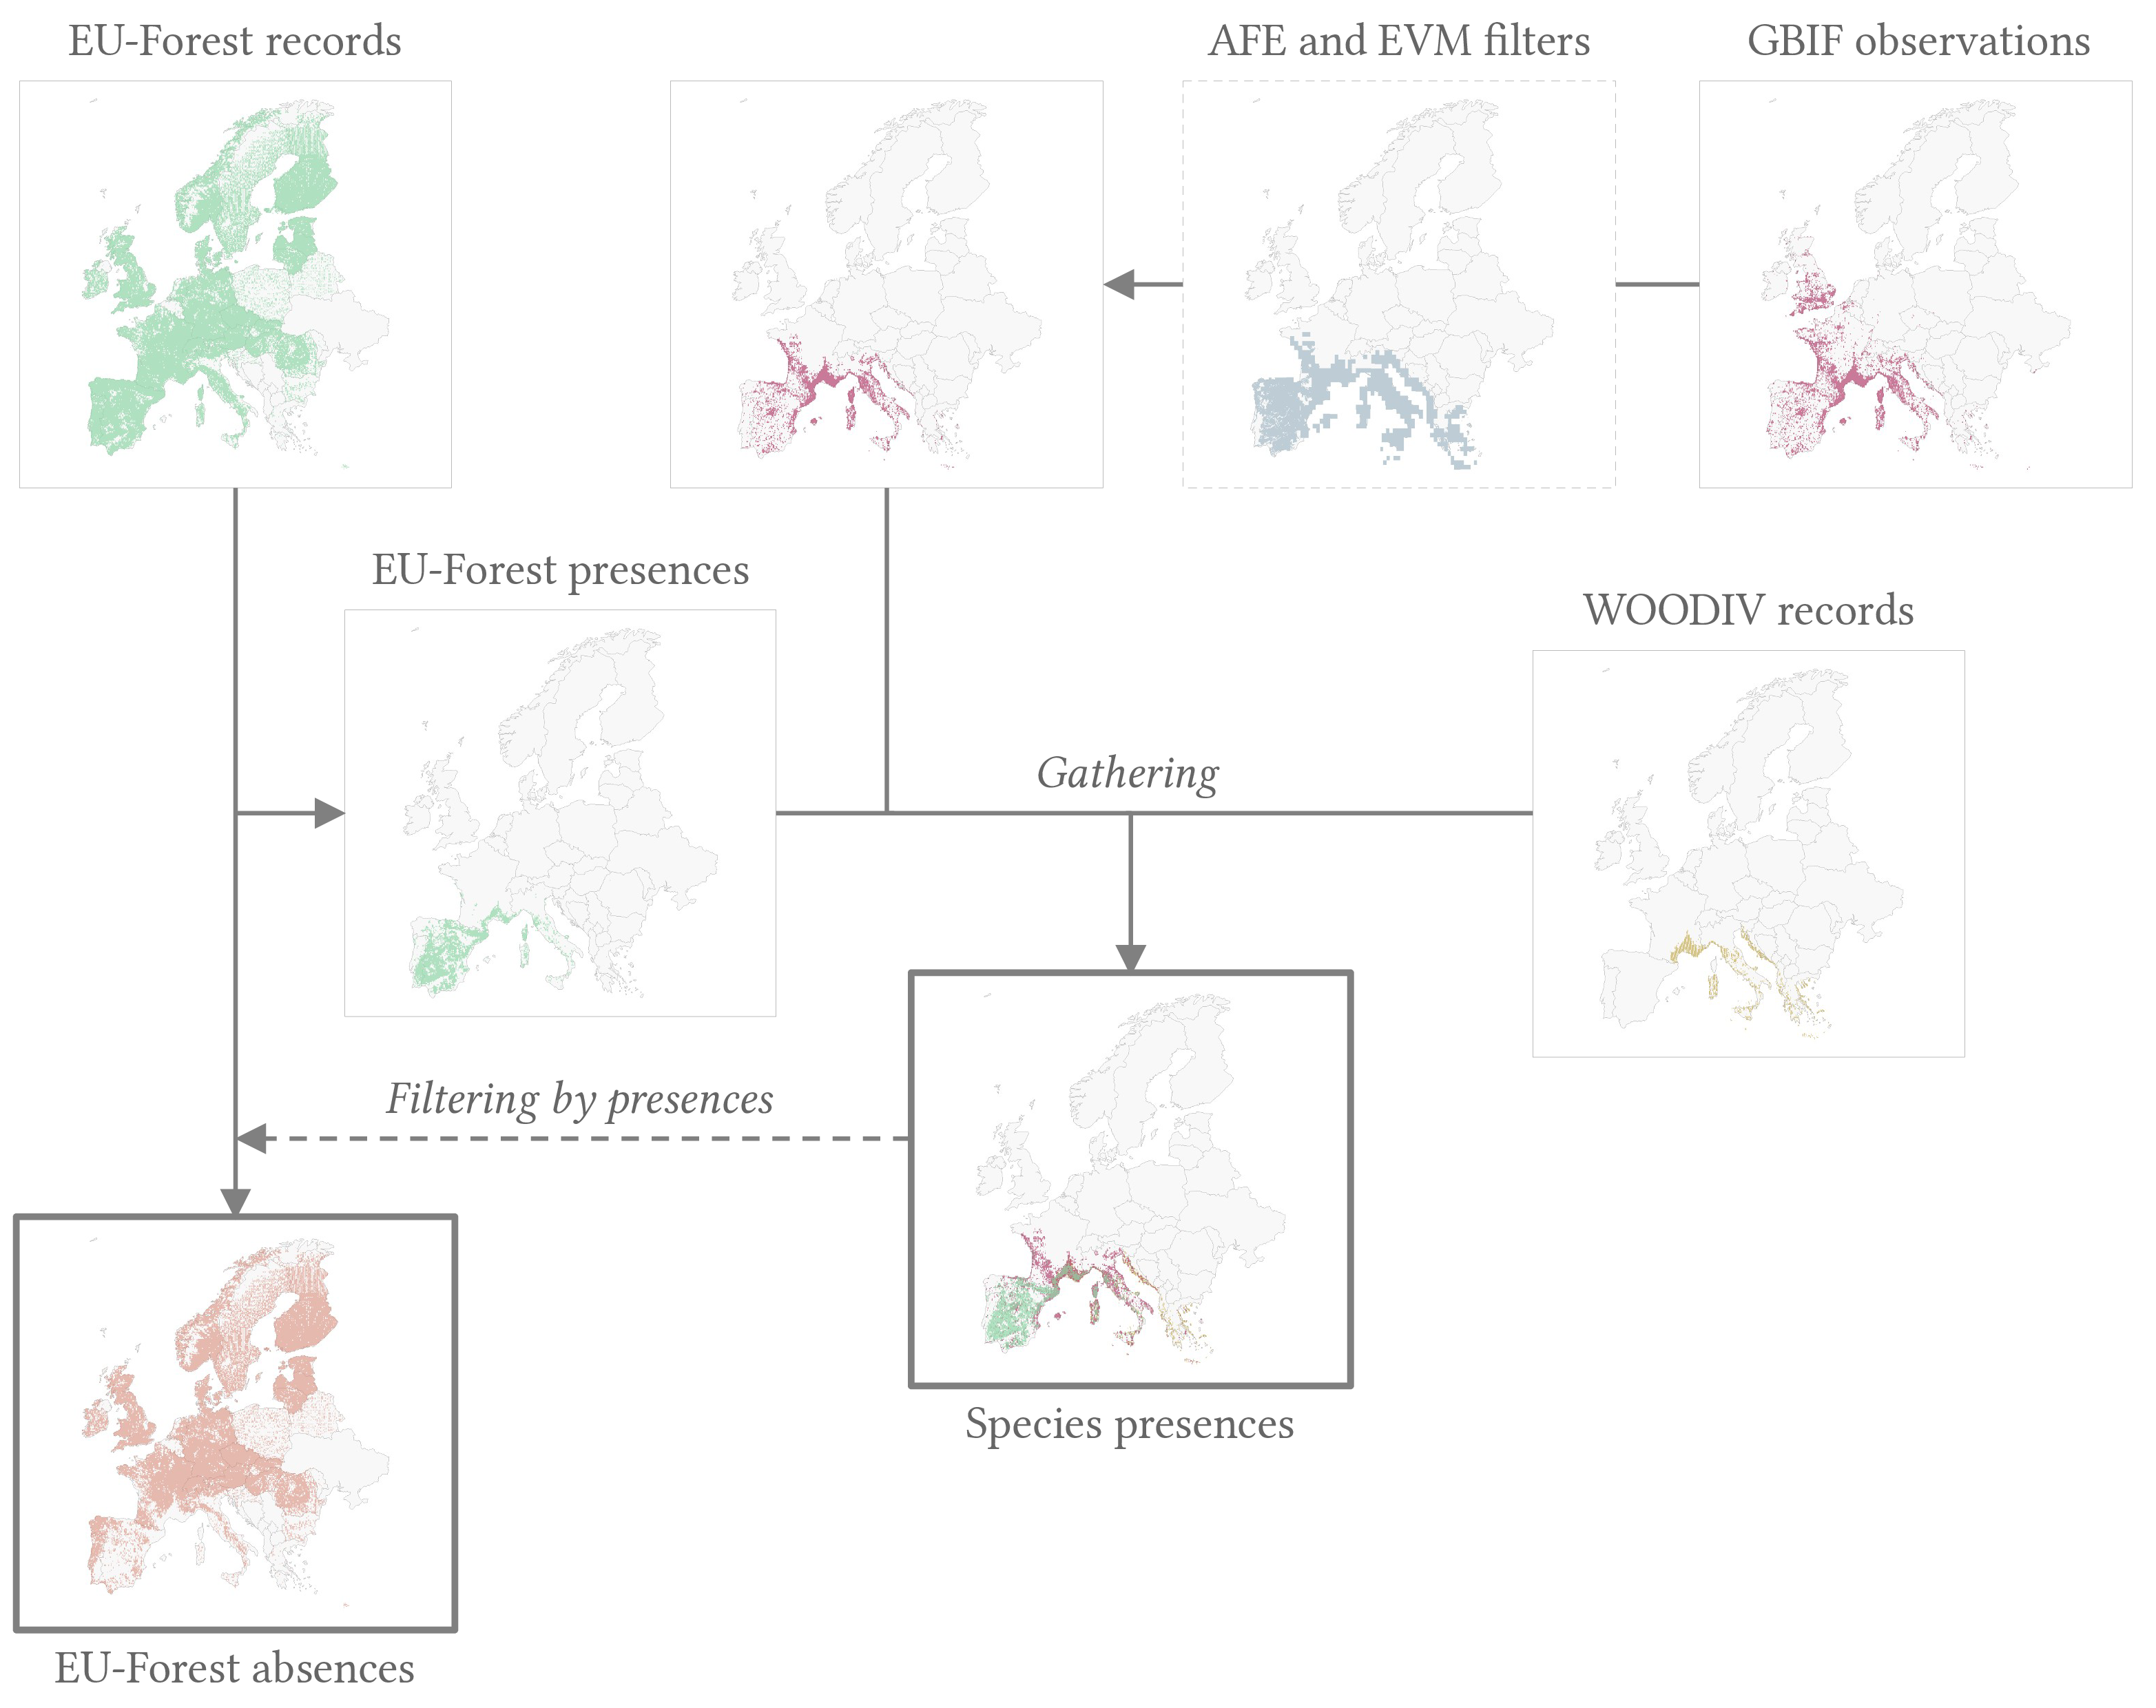
\includegraphics{figs/files/occurrence_processing} 

}

\caption{Processing of holm oak occurrence records. GBIF: Global Biodiversity Information Facility, AFE: Atlas Flora Europeae, EVM: EuroVegMap.}\label{fig:occ_processing}
\end{figure}
\end{landscape}

\newpage

\newpage

\hypertarget{appendixC}{%
\section{Supplementary Appendix C: Species
distributions}\label{appendixC}}

\renewcommand*\thetable{C.\arabic{table}}
\renewcommand*\thefigure{C.\arabic{figure}}

\setcounter{figure}{0}
\setcounter{table}{0}

\pagenumbering{arabic}
\renewcommand*{\thepage}{C--\arabic{page}}

\begin{figure}
\centering
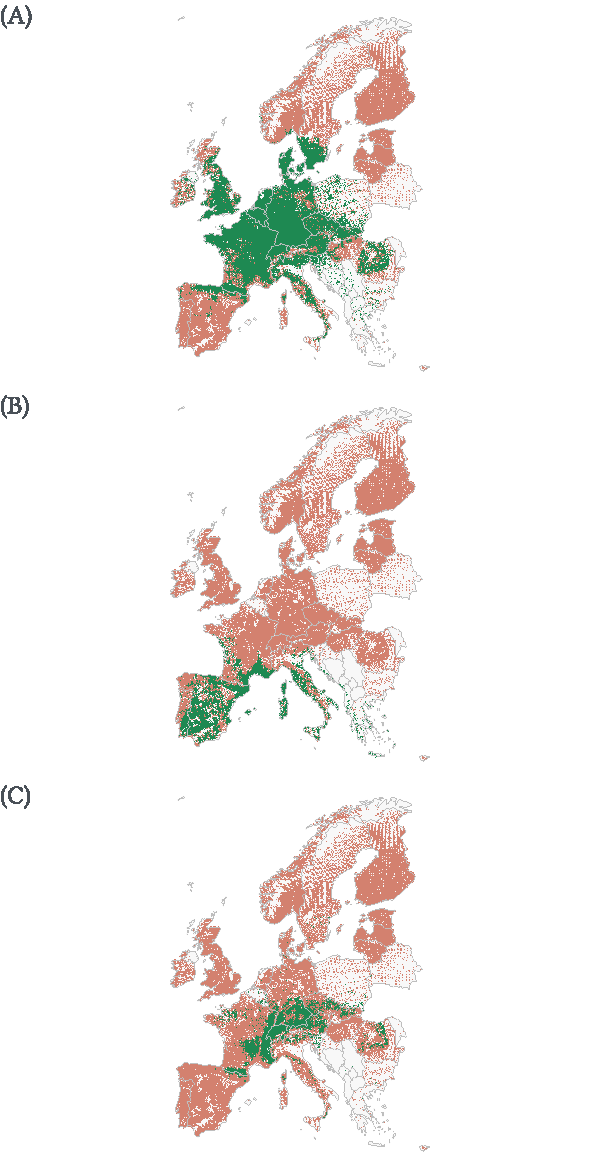
\includegraphics{figs/distributionmaps.pdf}
\caption{Species distributions of \textbf{(A)} beech, \textbf{(B)} holm
oak and \textbf{(C)} silver fir. Green cells are \(0.1^\circ\) cells
where species is present, orange cells where species is supposed to be
absent.}
\end{figure}

\newpage

\hypertarget{appendixD}{%
\section{Supplementary Appendix D: Handling constraints in
CMA-ES}\label{appendixD}}

\renewcommand*\thetable{D.\arabic{table}}
\renewcommand*\thefigure{D.\arabic{figure}}

\setcounter{figure}{0}
\setcounter{table}{0}

\pagenumbering{arabic}
\renewcommand*{\thepage}{D--\arabic{page}}

\hfill \break

\hypertarget{box-constraint-handling}{%
\subsection{Box constraint handling}\label{box-constraint-handling}}

With this constraint handling - implemented by default in the R package
\emph{cmaes} (\protect\hyperlink{ref-Trautmann2011}{Trautmann \emph{et
al.} 2011}) - each evaluated solution is guaranteed to lie within the
feasible space. Let's say we have a parameter vector \(x\). For each
parameter \(x_i\), we have a lower bound \(lb_i\) and an upper bound
\(ub_i\). If a parameter \(x_i\) violates one of this bound, we set
\(x_i\) to a new value \(x_i^{repaired}\) equal to the closest boundary
value (\(lb_i\) or \(ub_i\)). We thus obtained a new parameter set
\(x^{repaired}\), with a minimal \(\|x-x^{repaired}\|\) value. This new
feasible solution \(x^{repaired}\) is used for the evaluation of the
objective function \(AUC_{model}(x^{repaired})\), and to compute a
penalty term
\(pen=\sum\limits_{i}(x_i-x_i^{repaired})^2=\|x^{repaired}-x\|^2\). Then
\(x^{repaired}\) is discarded, and the algorithm computes the penalized
objective function of \(x^{repaired}\) as follows:
\(AUC_{model}(x)=AUC_{model}(x^{repaired})+pen\). This boundary handling
could be improved with adaptive weights (see
\protect\hyperlink{ref-Hansen2009}{Hansen \emph{et al.} 2009}).

\hypertarget{ecological-infeasibility-constraint}{%
\subsection{Ecological infeasibility
constraint}\label{ecological-infeasibility-constraint}}

We added a simple way to handle ecological constraint (e.g.~unfolding
before flowering in beech mixed bud) with a death penalty. When a
parameter vector \(x\) violates a constraint, it is rejected and
generated again. The main drawback of this approach is that CMA-ES does
not use information from unfeasible points. An other approach could be
to set \(AUC_{model}(x)=0\). However, as our feasible space was large,
the death penalty constraint worked well in our case.

\newpage

\hypertarget{appendixE}{%
\section{Supplementary Appendix E: holm oak and silver fir
calibrations}\label{appendixE}}

\renewcommand*\thetable{E.\arabic{table}}
\renewcommand*\thefigure{E.\arabic{figure}}

\setcounter{figure}{0}
\setcounter{table}{0}

\pagenumbering{arabic}
\renewcommand*{\thepage}{E--\arabic{page}}

\hfill \break

\begin{figure}[H]

{\centering 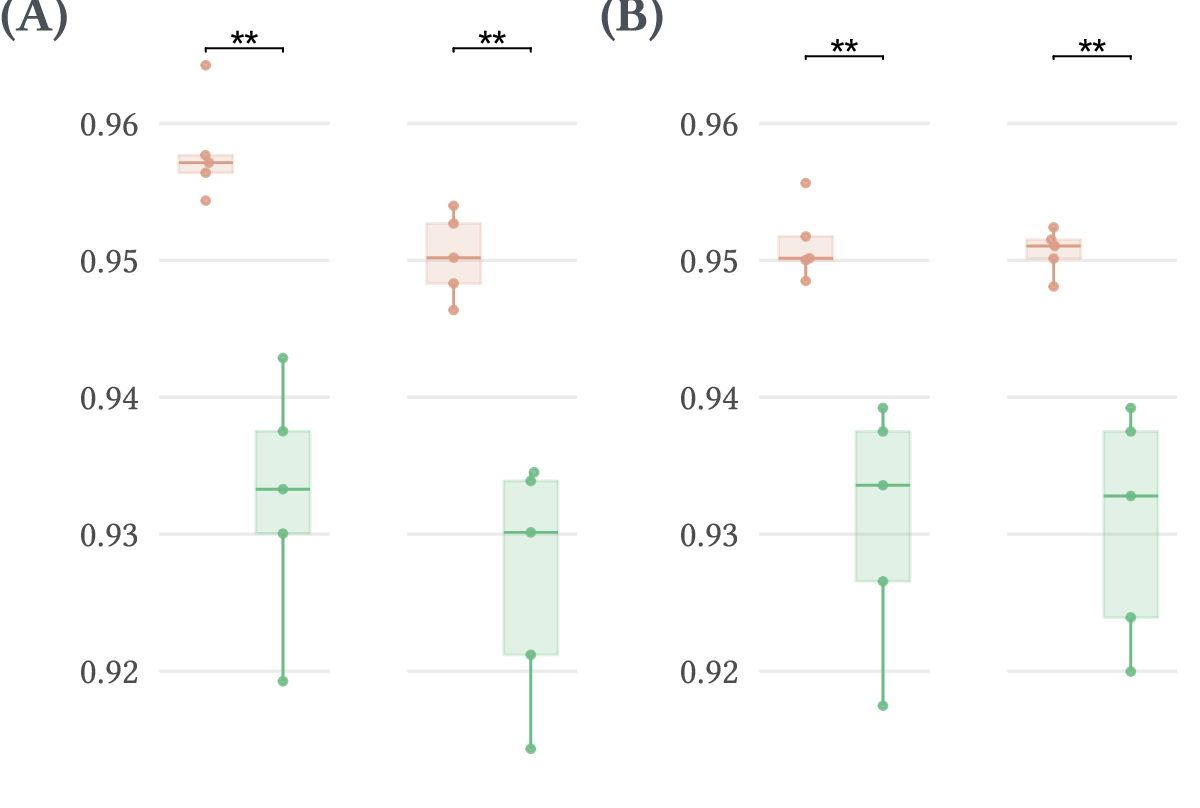
\includegraphics{figs/comparisonquercusABCCMAES} 

}

\caption{Comparison of CMA-ES and ABC-rejection methods, with two holm oak occurrence subsets, on \textbf{(A)} calibration AUC (only calibration points) and \textbf{(B)} total AUC (every presence/absence points). Each point is a calibration run. The black horizontal bars represent the pairwise Mann–Whitney tests between the two methods on the same subset. CMA-ES is red and ABC green.}\label{fig:comparisonquercusABCCMAES}
\end{figure}

\begin{figure}[H]

{\centering 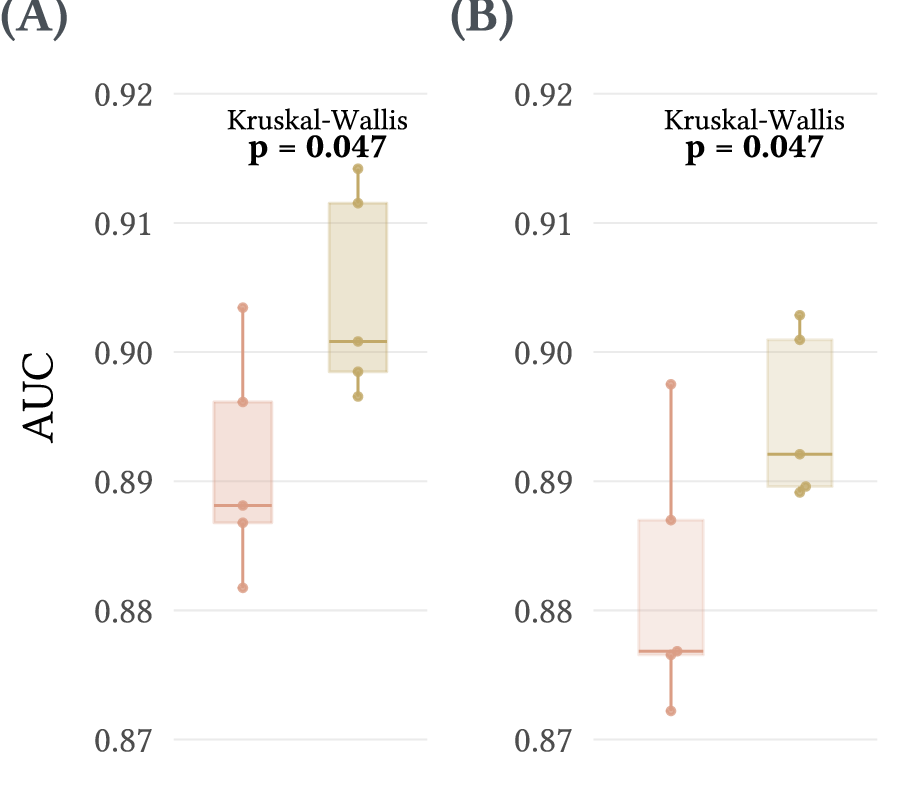
\includegraphics{figs/calibCMAESabies} 

}

\caption{CMA-ES calibration using the PHENOFIT model and silver fir: \textbf{(A)} calibration AUC (only calibration cells) and \textbf{(B)} total AUC (every presence/absence cells). Each color is a different sub-sampling of occurrence data, each point is a calibration run. The black horizontal bars represent the pairwise Mann–Whitney tests between the two subsets.}\label{fig:calibCMAESabies}
\end{figure}

\newpage

\hypertarget{appendixF}{%
\section{Supplementary Appendix F: Raw model outputs}\label{appendixF}}

\renewcommand*\thetable{F.\arabic{table}}
\renewcommand*\thefigure{F.\arabic{figure}}

\setcounter{figure}{0}
\setcounter{table}{0}

\pagenumbering{arabic}
\renewcommand*{\thepage}{F--\arabic{page}}

\hfill \break

\begin{figure}[H]

{\centering 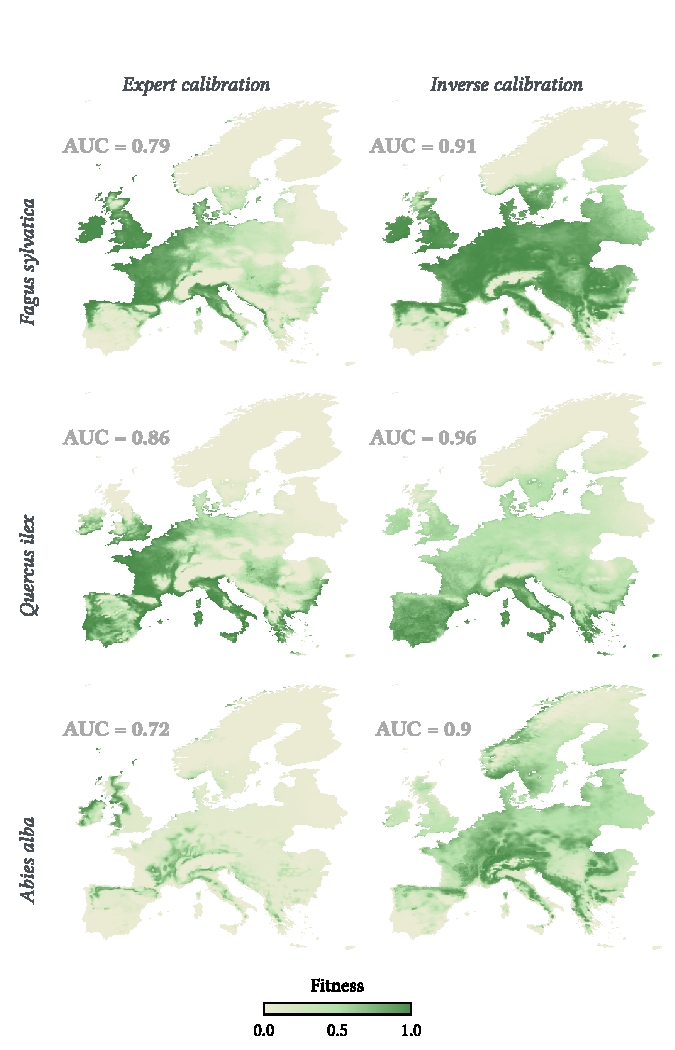
\includegraphics{figs/phenofit_output_maps} 

}

\caption{Fitness index predicted by PHENOFIT with the forward and the backward calibrations.}\label{fig:phenofit_output_maps}
\end{figure}

\begin{figure}[H]

{\centering 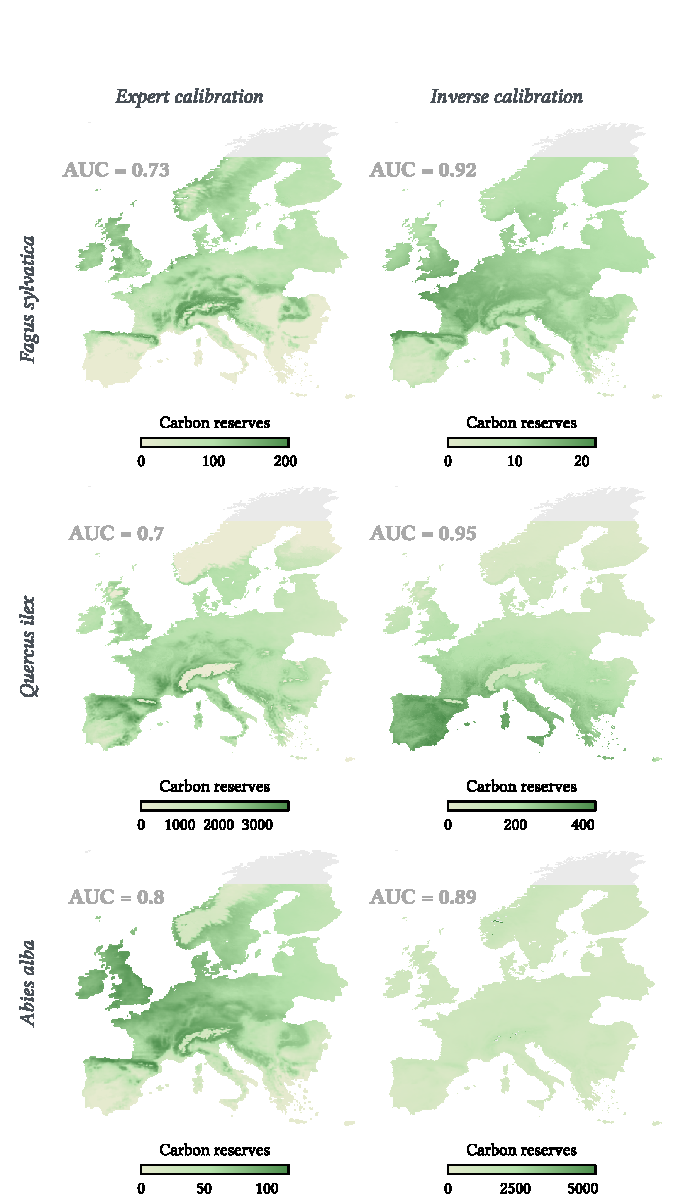
\includegraphics{figs/best_forward_maps} 

}

\caption{Carbon reserves predicted by CASTANEA with the forward and the backward calibrations.}\label{fig:best_forward_maps}
\end{figure}

\newpage

\hypertarget{appendixG}{%
\section{Supplementary Appendix G: Leaf unfolding
submodel}\label{appendixG}}

\renewcommand*\thetable{G.\arabic{table}}
\renewcommand*\thefigure{G.\arabic{figure}}

\setcounter{figure}{0}
\setcounter{table}{0}

\pagenumbering{arabic}
\renewcommand*{\thepage}{G--\arabic{page}}

\hfill \break

\hypertarget{fagus-sylvatica-leaf-unfolding-submodel}{%
\subsection{Fagus sylvatica leaf unfolding
submodel}\label{fagus-sylvatica-leaf-unfolding-submodel}}

This model, called UniChill (\protect\hyperlink{ref-Chuine2000}{Chuine
2000}), is a sequential two-phase model (endodormancy and ecodormancy
phases).\\
The endodormancy phase begins at day \(t_0\). The daily rate of chilling
\(R_c\) is defined as a threshold function of the daily mean temperature
\(T_d\): \[ R_c(T_d) = \left\{
\begin{array}{ll}
      0 & T_d \geq T_b \\
      1 & T_d < T_b \\
\end{array} 
\right. \] where \(T_b\) is the threshold temperature below which the
bud accumulates chilling units.\\
The endodormancy releases at day \(t_c\) when the accumulated rate of
chilling has reached the level \(C_{crit}\):
\[\sum\limits_{t_0}^{t_c} R_c(T_d) \geq C_{crit} \] Then, the
ecodormancy phase begins. The daily rate of forcing \(R_f\) is defined
as a sigmoid function of the daily mean temperature \(T_d\):
\[R_f(T_d) = \frac{1}{1 + e^{-d_T(T_d-T_{50})}} \] where \(d_T\) is the
slope and \(T_{50}\) the mid-response temperature. Bud break occurs at
day \(t_f\) when the accumulated rate of forcing has reached the level
\(F_{crit}\): \[\sum\limits_{t_c}^{t_f} R_f(T_d) \geq F_{crit} \] Thus,
the UniChill model has 6 parameters: \(t_0\), \(T_b\) and \(C_{crit}\)
for the first phase, \(d_T\), \(T_{50}\) and \(F_{crit}\) for the second
phase.

\begin{figure}[H]

{\centering 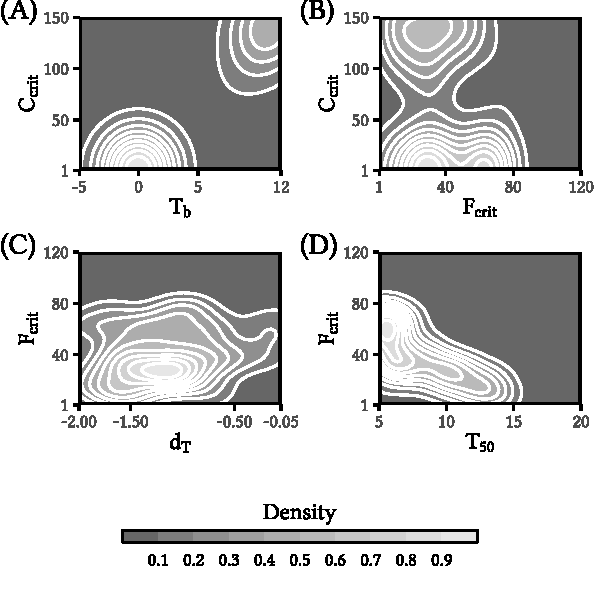
\includegraphics{figs/leafpardensity} 

}

\caption{Beech leaf unfolding model parameter density. Y-axis and X-axis limits are lower and upper bounds used during calibration.}\label{fig:leafpardensity}
\end{figure}

\begin{figure}[H]

{\centering 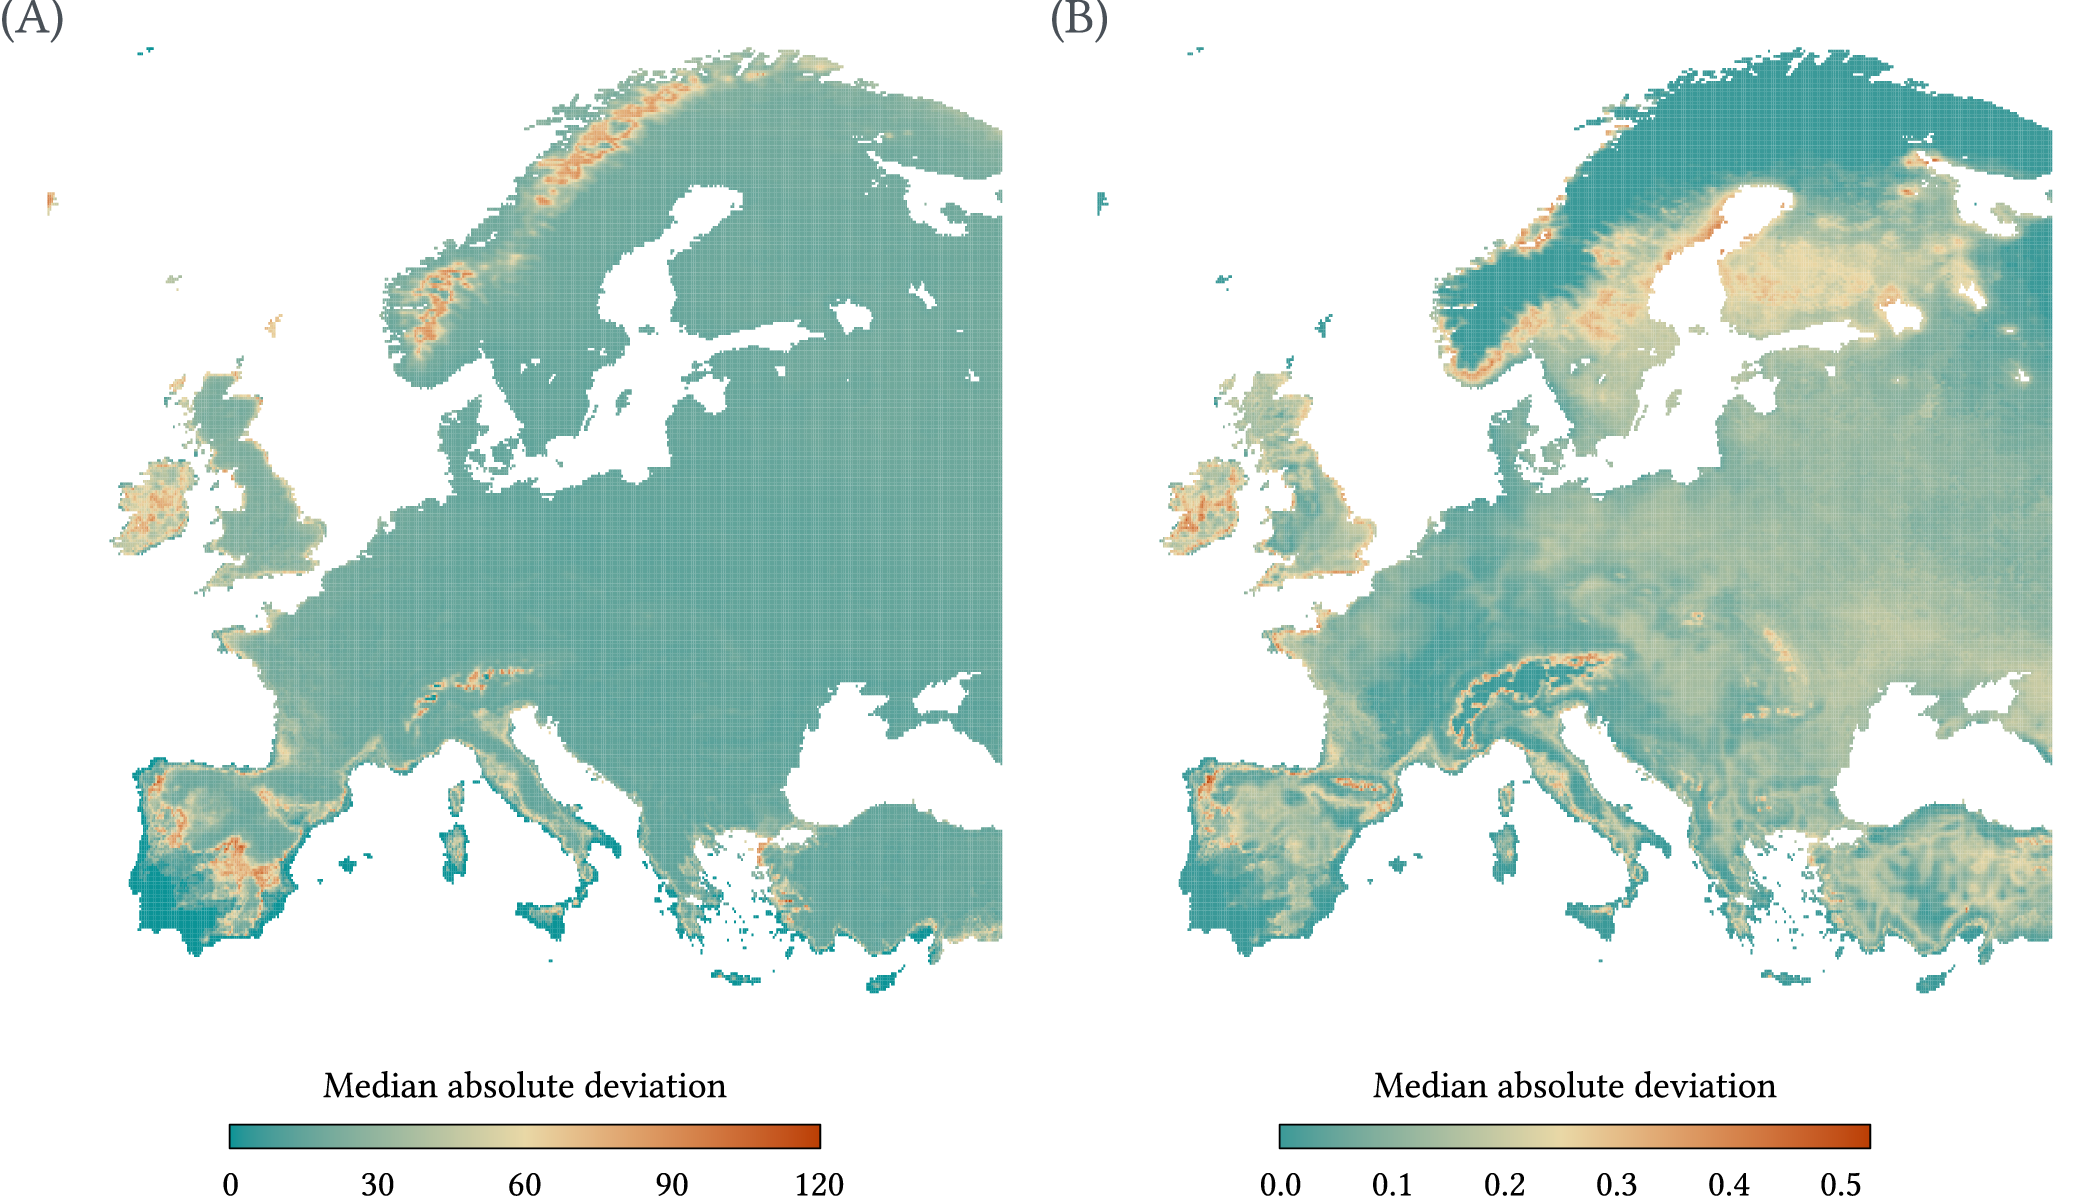
\includegraphics{figs/consensusfitnessmap} 

}

\caption{Median absolute deviation of beech \textbf{(A)} leaf unfolding date and \textbf{(B)} fitness, predicted with 100 calibrated parameter sets of PHENOFIT.}\label{fig:consensusfitnessmap}
\end{figure}

The median standard deviation of unfolding date across Europe was about
15.4 days. On beech presence points, it was about 16.2 days. Nearly
90.3\% of cells had a median absolute deviation lower than 30 days
(\hyperref[fig:consensusfitnessmap]{Figure D.2.A.}). The median standard
deviation of fitness across Europe was about 0.148. On beech presence
points, it was about 0.153. Nearly 46.4\% and 91.5\% of total cells had
a median absolute deviation lower than 0.1 and 0.2 respectively
(\hyperref[fig:consensusfitnessmap]{Figure D.2.B.}).

\begin{figure}[H]

{\centering 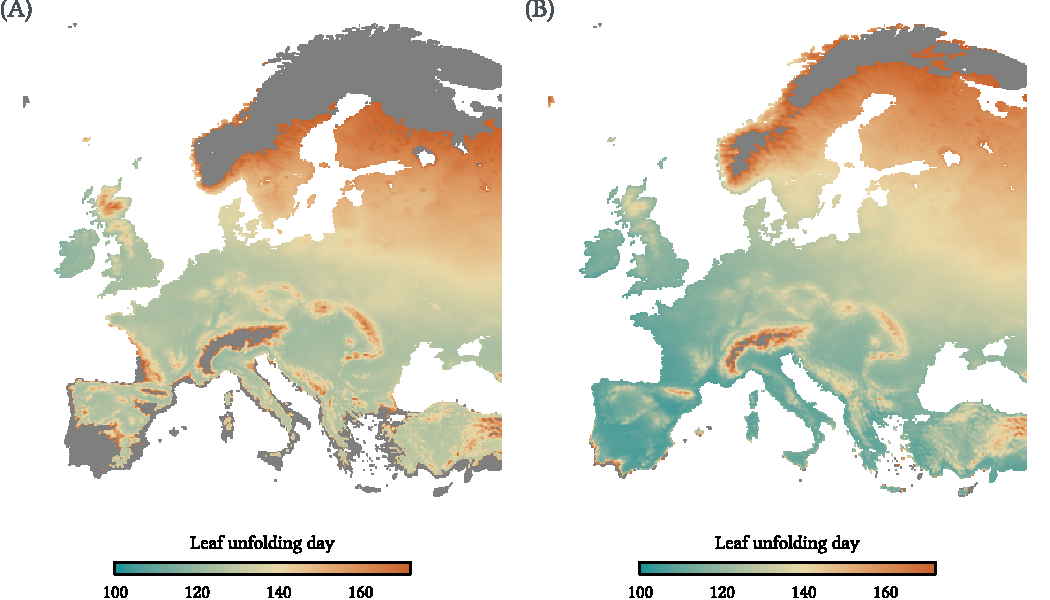
\includegraphics{figs/unfoldingdatesbackforw} 

}

\caption{Mean leaf unfolding day of beech with \textbf{(A)} best CMA-ES calibrated parameters and \textbf{(B)} classical (forward) parameters. Values above June solstice day are in grey. Note that PHENOFIT model assign a value of 365 when unfolding has not happened at all due to climate conditions.}\label{fig:unfoldingdatesbackforw}
\end{figure}





\newpage
\singlespacing
\printbibliography

\end{document}
